%  A simple AAU report template.
%  2015-05-08 v. 1.2.0
%  Copyright 2010-2015 by Jesper Kjær Nielsen <jkn@es.aau.dk>
%
%  This is free software: you can redistribute it and/or modify
%  it under the terms of the GNU General Public License as published by
%  the Free Software Foundation, either version 3 of the License, or
%  (at your option) any later version.
%
%  This is distributed in the hope that it will be useful,
%  but WITHOUT ANY WARRANTY; without even the implied warranty of
%  MERCHANTABILITY or FITNESS FOR A PARTICULAR PURPOSE.  See the
%  GNU General Public License for more details.
%
%  You can find the GNU General Public License at <http://www.gnu.org/licenses/>.
%
%  A simple AAU report template.
%  2015-05-08 v. 1.2.0
%  Copyright 2010-2015 by Jesper Kjær Nielsen <jkn@es.aau.dk>
%
%  This is free software: you can redistribute it and/or modify
%  it under the terms of the GNU General Public License as published by
%  the Free Software Foundation, either version 3 of the License, or
%  (at your option) any later version.
%
%  This is distributed in the hope that it will be useful,
%  but WITHOUT ANY WARRANTY; without even the implied warranty of
%  MERCHANTABILITY or FITNESS FOR A PARTICULAR PURPOSE.  See the
%  GNU General Public License for more details.
%
%  You can find the GNU General Public License at <http://www.gnu.org/licenses/>.
%
\documentclass[11pt,twoside,a4paper,openany]{report}
%%%%%%%%%%%%%%%%%%%%%%%%%%%%%%%%%%%%%%%%%%%%%%%%
% Language, Encoding and Fonts
% http://en.wikibooks.org/wiki/LaTeX/Internationalization
%%%%%%%%%%%%%%%%%%%%%%%%%%%%%%%%%%%%%%%%%%%%%%%%
% Select encoding of your inputs. Depends on
% your operating system and its default input
% encoding. Typically, you should use
%   Linux  : utf8 (most modern Linux distributions)
%            latin1 
%   Windows: ansinew
%            latin1 (works in most cases)
%   Mac    : applemac
% Notice that you can manually change the input
% encoding of your files by selecting "save as"
% an select the desired input encoding. 
\usepackage[utf8]{inputenc}
% Make latex understand and use the typographic
% rules of the language used in the document.
\usepackage[danish,english]{babel}
% hide border around links
\usepackage[hidelinks]{hyperref}
% Use the palatino font
\usepackage[sc]{mathpazo}
\linespread{1.05}         % Palatino needs more leading (space between lines)
% Choose the font encoding
\usepackage[T1]{fontenc}
%%%%%%%%%%%%%%%%%%%%%%%%%%%%%%%%%%%%%%%%%%%%%%%%
% Graphics and Tables
% http://en.wikibooks.org/wiki/LaTeX/Importing_Graphics
% http://en.wikibooks.org/wiki/LaTeX/Tables
% http://en.wikibooks.org/wiki/LaTeX/Colors
%%%%%%%%%%%%%%%%%%%%%%%%%%%%%%%%%%%%%%%%%%%%%%%%
% load a colour package
\usepackage{xcolor}
\definecolor{aaublue}{RGB}{33,26,82}% dark blue
% The standard graphics inclusion package
\usepackage{graphicx}
% Set up how figure and table captions are displayed
\usepackage{caption}
\captionsetup{%
  font=footnotesize,% set font size to footnotesize
  labelfont=bf % bold label (e.g., Figure 3.2) font
}
% Make the standard latex tables look so much better
\usepackage{array,booktabs}
% Enable the use of frames around, e.g., theorems
% The framed package is used in the example environment
\usepackage{framed}

%%%%%%%%%%%%%%%%%%%%%%%%%%%%%%%%%%%%%%%%%%%%%%%%
% Mathematics
% http://en.wikibooks.org/wiki/LaTeX/Mathematics
%%%%%%%%%%%%%%%%%%%%%%%%%%%%%%%%%%%%%%%%%%%%%%%%
% Defines new environments such as equation,
% align and split 
\usepackage{amsmath}
% Adds new math symbols
\usepackage{amssymb}
% Use theorems in your document
% The ntheorem package is also used for the example environment
% When using thmmarks, amsmath must be an option as well. Otherwise \eqref doesn't work anymore.
\usepackage[framed,amsmath,thmmarks]{ntheorem}

%%%%%%%%%%%%%%%%%%%%%%%%%%%%%%%%%%%%%%%%%%%%%%%%
% Page Layout
% http://en.wikibooks.org/wiki/LaTeX/Page_Layout
%%%%%%%%%%%%%%%%%%%%%%%%%%%%%%%%%%%%%%%%%%%%%%%%
% Change margins, papersize, etc of the document
\usepackage[
  inner=28mm,% left margin on an odd page
  outer=41mm,% right margin on an odd page
  ]{geometry}
% Modify how \chapter, \section, etc. look
% The titlesec package is very configureable [display] \chaptertitlename\
\usepackage{titlesec}
\titleformat{\chapter}{\normalfont\huge\bfseries}{ \thechapter}{20pt}{\Huge}
\titleformat*{\section}{\normalfont\Large\bfseries}
\titleformat*{\subsection}{\normalfont\large\bfseries}
\titleformat*{\subsubsection}{\normalfont\normalsize\bfseries}
%\titleformat*{\paragraph}{\normalfont\normalsize\bfseries}
%\titleformat*{\subparagraph}{\normalfont\normalsize\bfseries}

% Clear empty pages between chapters
\let\origdoublepage\cleardoublepage
\newcommand{\clearemptydoublepage}{%
  \clearpage
  {\pagestyle{empty}\origdoublepage}%
}
\let\cleardoublepage\clearemptydoublepage

% Change the headers and footers
\usepackage{fancyhdr}
\pagestyle{fancy}
\fancyhf{} %delete everything
\renewcommand{\headrulewidth}{0pt} %remove the horizontal line in the header
\fancyhead[RE]{\small\nouppercase\leftmark} %even page - chapter title
\fancyhead[LO]{\small\nouppercase\rightmark} %uneven page - section title
\fancyhead[LE,RO]{\thepage} %page number on all pages
% Do not stretch the content of a page. Instead,
% insert white space at the bottom of the page
\raggedbottom
% Enable arithmetics with length. Useful when
% typesetting the layout.
\usepackage{calc}

%%%%%%%%%%%%%%%%%%%%%%%%%%%%%%%%%%%%%%%%%%%%%%%%
% Bibliography
% http://en.wikibooks.org/wiki/LaTeX/Bibliography_Management
%%%%%%%%%%%%%%%%%%%%%%%%%%%%%%%%%%%%%%%%%%%%%%%%
\usepackage[backend=bibtex,
  bibencoding=utf8
  ]{biblatex}
\addbibresource{bib/mybib}

%%%%%%%%%%%%%%%%%%%%%%%%%%%%%%%%%%%%%%%%%%%%%%%%
% Misc
%%%%%%%%%%%%%%%%%%%%%%%%%%%%%%%%%%%%%%%%%%%%%%%%
% Add bibliography and index to the table of
% contents
\usepackage[nottoc]{tocbibind}
% Add the command \pageref{LastPage} which refers to the
% page number of the last page
\usepackage{lastpage}
% Add todo notes in the margin of the document
\usepackage[
%  disable, %turn off todonotes
  colorinlistoftodos, %enable a coloured square in the list of todos
  textwidth=\marginparwidth, %set the width of the todonotes
  textsize=scriptsize, %size of the text in the todonotes
  ]{todonotes}
% For typesetting C codes
\usepackage{listings}
%%%%%%%%%%%%%%%%%%%%%%%%%%%%%%%%%%%%%%%%%%%%%%%%
% Hyperlinks
% http://en.wikibooks.org/wiki/LaTeX/Hyperlinks
%%%%%%%%%%%%%%%%%%%%%%%%%%%%%%%%%%%%%%%%%%%%%%%%
% Enable hyperlinks and insert info into the pdf
% file. Hypperref should be loaded as one of the 
% last packages
\usepackage{hyperref}
\usepackage{xcolor} %custom colours
\usepackage{mdframed} %nice frames

\definecolor{light-gray}{gray}{0.95} %the shade of grey that stack exchange uses
\definecolor{light-blue}{HTML}{2E86C1} 
\renewcommand{\labelitemii}{$\star$}
\hypersetup{%
	pdfpagelabels=true,%
	plainpages=false,%
	pdfauthor={Author(s)},%
	pdftitle={Title},%
	pdfsubject={Subject},%
	bookmarksnumbered=true,%
	colorlinks=false,%
	citecolor=black,%
	filecolor=black,%
	linkcolor=black,% you should probably change this to black before printing
	urlcolor=black,%
	pdfstartview=FitH%
}
% for symb
\usepackage{gensymb}  
\usepackage{float}  % package inclusion and set up of the document
% see, e.g., http://en.wikibooks.org/wiki/LaTeX/Formatting#Hyphenation
% for more information on word hyphenation
\hyphenation{ex-am-ple hy-phen-a-tion short}
\hyphenation{long la-tex}
% 
%  A simple AAU report template.
%  2015-05-08 v. 1.2.0
%  Copyright 2010-2015 by Jesper Kjær Nielsen <jkn@es.aau.dk>
%
%  This is free software: you can redistribute it and/or modify
%  it under the terms of the GNU General Public License as published by
%  the Free Software Foundation, either version 3 of the License, or
%  (at your option) any later version.
%
%  This is distributed in the hope that it will be useful,
%  but WITHOUT ANY WARRANTY; without even the implied warranty of
%  MERCHANTABILITY or FITNESS FOR A PARTICULAR PURPOSE.  See the
%  GNU General Public License for more details.
%
%  You can find the GNU General Public License at <http://www.gnu.org/licenses/>.
%
%
%
% see, e.g., http://en.wikibooks.org/wiki/LaTeX/Customizing_LaTeX#New_commands
% for more information on how to create macros

%%%%%%%%%%%%%%%%%%%%%%%%%%%%%%%%%%%%%%%%%%%%%%%%
% Macros for the titlepage
%%%%%%%%%%%%%%%%%%%%%%%%%%%%%%%%%%%%%%%%%%%%%%%%
%Creates the aau titlepage
\newcommand{\aautitlepage}[3]{%
  {
    %set up various length
    \ifx\titlepageleftcolumnwidth\undefined
      \newlength{\titlepageleftcolumnwidth}
      \newlength{\titlepagerightcolumnwidth}
    \fi
    \setlength{\titlepageleftcolumnwidth}{0.5\textwidth-\tabcolsep}
    \setlength{\titlepagerightcolumnwidth}{\textwidth-2\tabcolsep-\titlepageleftcolumnwidth}
    %create title page
    \thispagestyle{empty}
    \noindent%
    \begin{tabular}{@{}ll@{}}
      \parbox{\titlepageleftcolumnwidth}{
        \iflanguage{danish}{%
          
\includegraphics[width=\titlepageleftcolumnwidth]{figures/aau_logo_da}
        }{%
          
\includegraphics[width=\titlepageleftcolumnwidth]{figures/aau_logo_en}
        }
      } &
      \parbox{\titlepagerightcolumnwidth}{\raggedleft\sf\small
        #2
      }\bigskip\\
       #1 &
      \parbox[t]{\titlepagerightcolumnwidth}{%
      \textbf{Abstract:}\bigskip\par
        \fbox{\parbox{\titlepagerightcolumnwidth-2\fboxsep-2\fboxrule}{%
          #3
        }}
      }\\
    \end{tabular}
    \vfill
    \iflanguage{danish}{%
      \noindent{\footnotesize\emph{Rapportens indhold er frit tilgængeligt, men offentliggørelse (med kildeangivelse) må kun ske efter aftale med forfatterne.}}
    }{%
      \noindent{\footnotesize\emph{The content of this report is freely available, but publication (with reference) may only be pursued due to agreement with the author.}}
    }
    \clearpage
  }
}

%Create english project info
\newcommand{\englishprojectinfo}[8]{%
  \parbox[t]{\titlepageleftcolumnwidth}{
    \textbf{Title:}\\ #1\bigskip\par
    \textbf{Theme:}\\ #2\bigskip\par
    \textbf{Project Period:}\\ #3\bigskip\par
    \textbf{Project Group:}\\ #4\bigskip\par
    \textbf{Participant(s):}\\ #5\bigskip\par
    \textbf{Supervisor(s):}\\ #6\bigskip\par
    \textbf{Copies:} #7\bigskip\par
    \textbf{Page Numbers:} \pageref{LastPage}\bigskip\par
    \textbf{Date of Completion:}\\ #8
  }
}

%Create danish project info
\newcommand{\danishprojectinfo}[8]{%
  \parbox[t]{\titlepageleftcolumnwidth}{
    \textbf{Titel:}\\ #1\bigskip\par
    \textbf{Tema:}\\ #2\bigskip\par
    \textbf{Projektperiode:}\\ #3\bigskip\par
    \textbf{Projektgruppe:}\\ #4\bigskip\par
    \textbf{Deltager(e):}\\ #5\bigskip\par
    \textbf{Vejleder(e):}\\ #6\bigskip\par
    \textbf{Oplagstal:} #7\bigskip\par
    \textbf{Sidetal:} \pageref{LastPage}\bigskip\par
    \textbf{Afleveringsdato:}\\ #8
  }
}

%%%%%%%%%%%%%%%%%%%%%%%%%%%%%%%%%%%%%%%%%%%%%%%%
% An example environment
%%%%%%%%%%%%%%%%%%%%%%%%%%%%%%%%%%%%%%%%%%%%%%%%
\theoremheaderfont{\normalfont\bfseries}
\theorembodyfont{\normalfont}
\theoremstyle{break}
\def\theoremframecommand{{\color{gray!50}\vrule width 5pt \hspace{5pt}}}
\newshadedtheorem{exa}{Example}[chapter]
\newenvironment{example}[1]{%
		\begin{exa}[#1]
}{%
		\end{exa}
}
% my new macros

\begin{document}
%frontmatter
\pagestyle{empty} %disable headers and footers
\pagenumbering{roman} %use roman page numbering in the frontmatter
%  A simple AAU report template.
%  2015-05-08 v. 1.2.0
%  Copyright 2010-2015 by Jesper Kjær Nielsen <jkn@es.aau.dk>
%
%  This is free software: you can redistribute it and/or modify
%  it under the terms of the GNU General Public License as published by
%  the Free Software Foundation, either version 3 of the License, or
%  (at your option) any later version.
%
%  This is distributed in the hope that it will be useful,
%  but WITHOUT ANY WARRANTY; without even the implied warranty of
%  MERCHANTABILITY or FITNESS FOR A PARTICULAR PURPOSE.  See the
%  GNU General Public License for more details.
%
%  You can find the GNU General Public License at <http://www.gnu.org/licenses/>.
%
\pdfbookmark[0]{Front page}{label:frontpage}%
\begin{titlepage}
  \addtolength{\hoffset}{0.5\evensidemargin-0.5\oddsidemargin} %set equal margins on the frontpage - remove this line if you want default margins
  \noindent%
  \begin{tabular}{@{}p{\textwidth}@{}}
    \toprule[2pt]
    \midrule
    \vspace{0.2cm}
    \begin{center}
    \Huge{\textbf{
      Report Title% insert your title here
    }}
    \end{center}
    \begin{center}
      \Large{
        - Subtitle -% insert your subtitle here
      }
    \end{center}
    \vspace{0.2cm}\\
    \midrule
    \toprule[2pt]
  \end{tabular}
  \vspace{4 cm}
  \begin{center}
    {\large
      Project Report%Insert document type (e.g., Project Report)
    }\\
    \vspace{0.2cm}
    {\Large
      Group Name/Number%Insert your group name or real names here
    }
  \end{center}
  \vfill
  \begin{center}
  Aalborg University\\
  Electronics and IT
  \end{center}
\end{titlepage}
\clearpage

\thispagestyle{empty}
{\small
\strut\vfill % push the content to the bottom of the page
\noindent Copyright \copyright{} Aalborg University 2015\par
\vspace{0.2cm}
\noindent Here you can write something about which tools and software you have used for typesetting the document, running simulations and creating figures. If you do not know what to write, either leave this page blank or have a look at the colophon in some of your books.
}
\clearpage


\pdfbookmark[0]{English title page}{label:titlepage_en}
\aautitlepage{%
  \englishprojectinfo{
    Project Title %title
  }{%
    Scientific Theme %theme
  }{%
    Fall Semester 2010 %project period
  }{%
    XXX % project group
  }{%
    %list of group members
    Author 1\\ 
    Author 2\\
    Author 3
  }{%
    %list of supervisors
    Supervisor 1\\
    Supervisor 2
  }{%
    1 % number of printed copies
  }{%
    \today % date of completion
  }%
}{%department and address
  \textbf{Electronics and IT}\\
  Aalborg University\\
  \href{http://www.aau.dk}{http://www.aau.dk}
}{% the abstract
  Here is the abstract
}

\cleardoublepage
\cleardoublepage
\pdfbookmark[0]{Contents}{label:contents}
\pagestyle{fancy} %enable headers and footers again
\tableofcontents
%\listoftodos
%\chapter*{Preface\markboth{Preface}{Preface}}\label{ch:preface}
\addcontentsline{toc}{chapter}{Preface}
Here is the preface. You should put your signatures at the end of the preface.

\vspace{\baselineskip}\hfill Aalborg University, \today
\vfill\noindent
\begin{minipage}[b]{0.45\textwidth}
 \centering
 \rule{\textwidth}{0.5pt}\\
  Author 1\\
 {\footnotesize <username1@XX.aau.dk>}
\end{minipage}
\hfill
\begin{minipage}[b]{0.45\textwidth}
 \centering
 \rule{\textwidth}{0.5pt}\\
  Author 2\\
 {\footnotesize <username2@XX.aau.dk>}
\end{minipage}
\vspace{3\baselineskip}
\begin{center}
\begin{minipage}[b]{0.45\textwidth}
 \centering
 \rule{\textwidth}{0.5pt}
  Author 3\\
 {\footnotesize <username3@XX.aau.dk>}
\end{minipage}
\end{center}

%\cleardoublepage
%mainmatter
\pagenumbering{arabic} %use arabic page numbering in the mainmatter
\chapter{Introduction}
\section{SECTION NAME}
\subsection{SUBSECTION NAME 1}
\paragraph{}WRITE HERE

\begin{figure}[H]
  \centering
    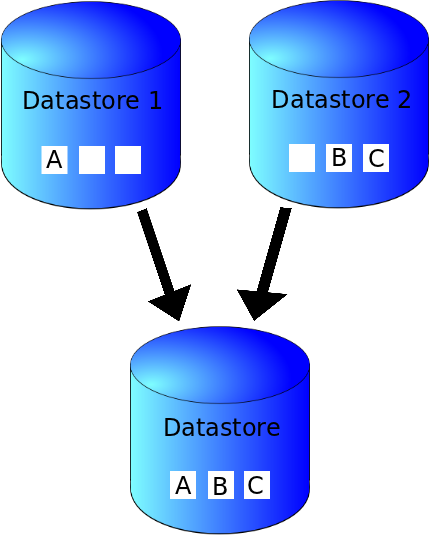
\includegraphics[height= 10cm, width=15cm]{project/images/data-sync}
  \caption{\textbf{IMAGE CAPTION}}
\end{figure}

\subsection{SUBSECTION NAME 2}
\paragraph{}WRITE HERE

\chapter{Circuit Schematics}\label{ch:chschematic}
\section{Arduino Pin Connections}
\begin{table}[H]
	\centering
	\begin{tabular}{|l|l|}
		\hline
		Pin of Arduino &Connected to\\
		\hline
		Digital I/O (2) &Trig of HC-SR04\\
		\hline
		Digital I/O (4)  &Echo of HC-SR04\\
		\hline
		Digital I/O (9) &Signal pin of Servo(orange)\\
		\hline
		Vcc &Vcc of HC-SR04 and Servo(Red)\\
		\hline
		GND Pin &GND of HC-SR04 and Servo(Black)\\
		\hline
	\end{tabular}
\end{table}
\section{Breadboard View}
\begin{figure}[H]
	\vfill
	\centering
	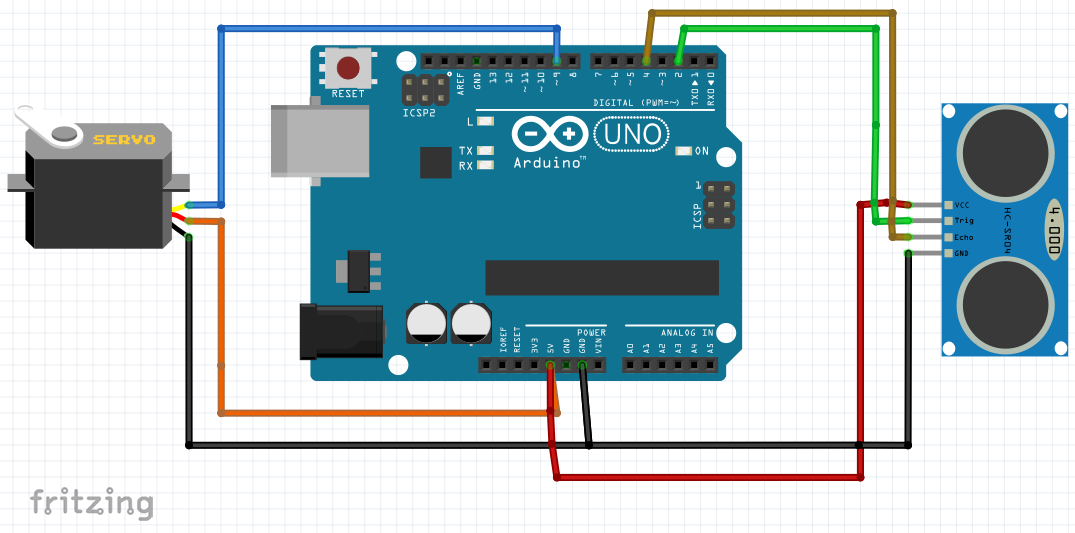
\includegraphics[width=\textwidth]{../Files/bboard}
	\caption{Circuit : Breadboard View}  \label{fig:bboard}
\end{figure}
\section{Schematic view}
\begin{figure}[H]
	\vfill
	\centering
	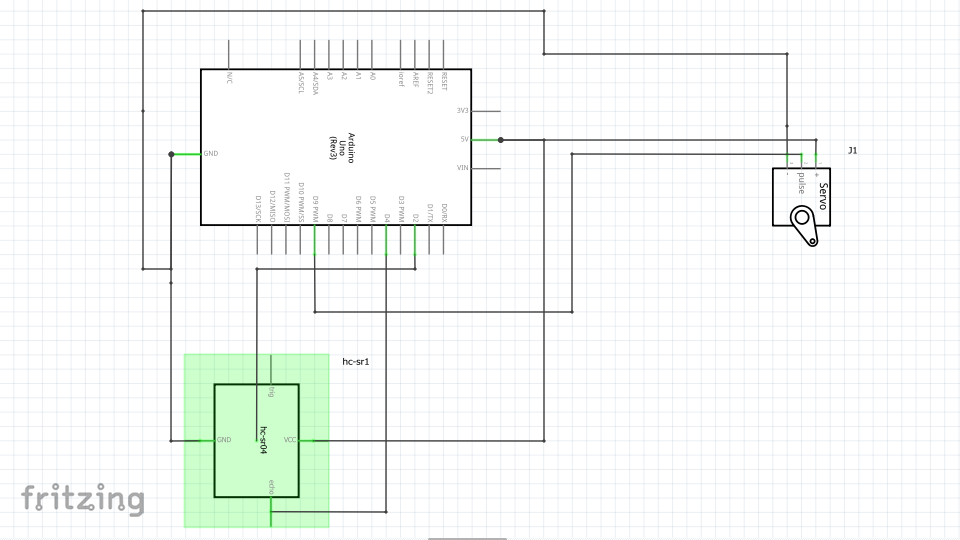
\includegraphics[width=\textwidth]{../Files/schematic}
	\caption{Circuit : Schematic view}  \label{fig:schematics}
\end{figure}
Above circuit schematics were obtained using the Fritzing software.\\
Once we decided the connections, we had to two more steps left before connecting the actual circuit: setting up the\textbf{ Development Environment} and \textbf{Circuit Simulation}.

\chapter{Development and Simulation}\label{ch:ch2label}
\section{Arduino IDE}
The code to be burnt to the program memory of an \arduino{} is written and compiled in the \emph{Arduino IDE}. The IDE also has a serial monitor, which displays values being recieved in real-time from the Arduino via serial communication through the serial port (COM ports). The IDE verifies for correct C/C++ syntax and compiles it, before linking it to Arduino Library files. This creates the \textit{hex} file that contains the code in binary form. It can either be uploaded to the board directly, which the IDE does with the help of the Bootloader program pre-installed on the Arduino, or it can be fed to a \emph{simulator}, which would simulate and show how the circuit would run and its associated parameters.
\begin{figure}[H]
	\vfill
	\centering
	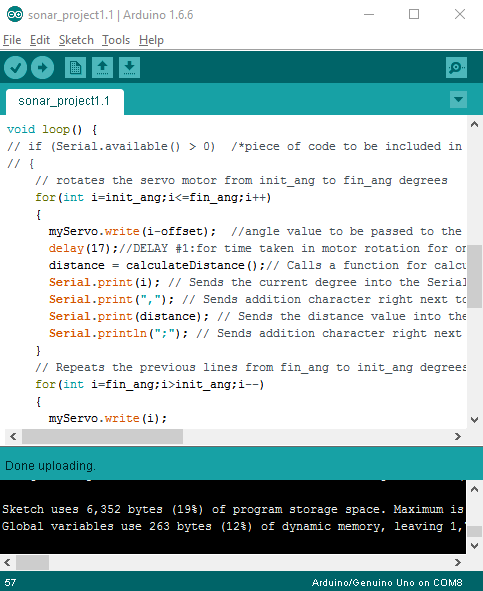
\includegraphics[width=0.5\textwidth]{../Files/IDE}
	\caption{The Arduino IDE}  \label{fig:IDE}
\end{figure}

%\cite{Madsen2010}, \cite{Oetiker2010} and \cite{Mittelbach2005}.

\clearpage

\section{Simulation with Proteus}
It is a good practice to simulate a circuit before connecting it, in order to avoid hardware damage/debug issues in a circuit beforehand. We used \emph{Proteus Professional} 8 for this purpose. Proteus has libraries for most commonly used electronics components, and it also allows us to make our own components, thanks to which we could download unavailable components from the internet, where many users have shared their own custom components.
\begin{figure}[H]
	\vfill
	\centering
	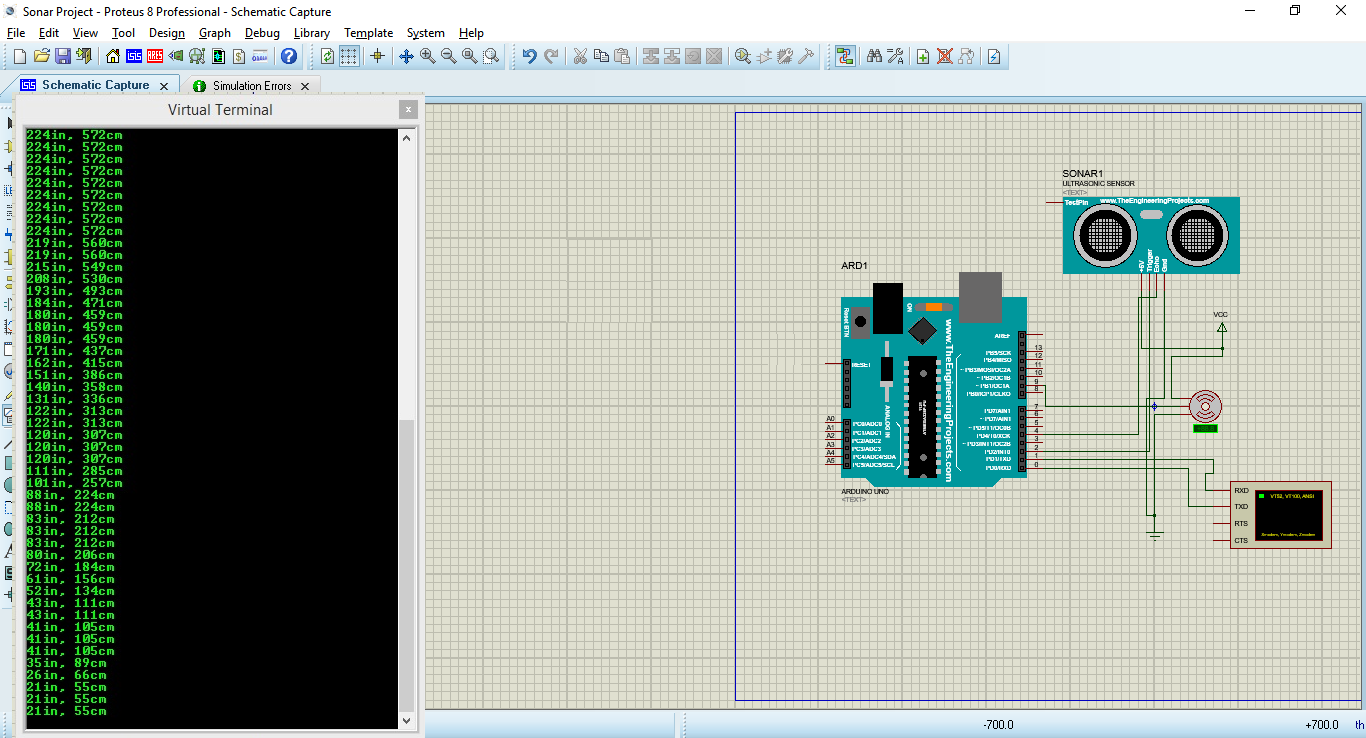
\includegraphics[width=0.7\textwidth]{../Files/proteus}
	\caption{The Proteus Simulator}  \label{fig:proteus}
\end{figure}

\section{Processing}
Processing is an interactive software to write programs with visual output. We have used Processing 3.2 for generating a 2D radar-map representation of the serial data being obtained from the Arduino through the computer's serial port.
\begin{figure}[H]
	\vfill
	\centering
	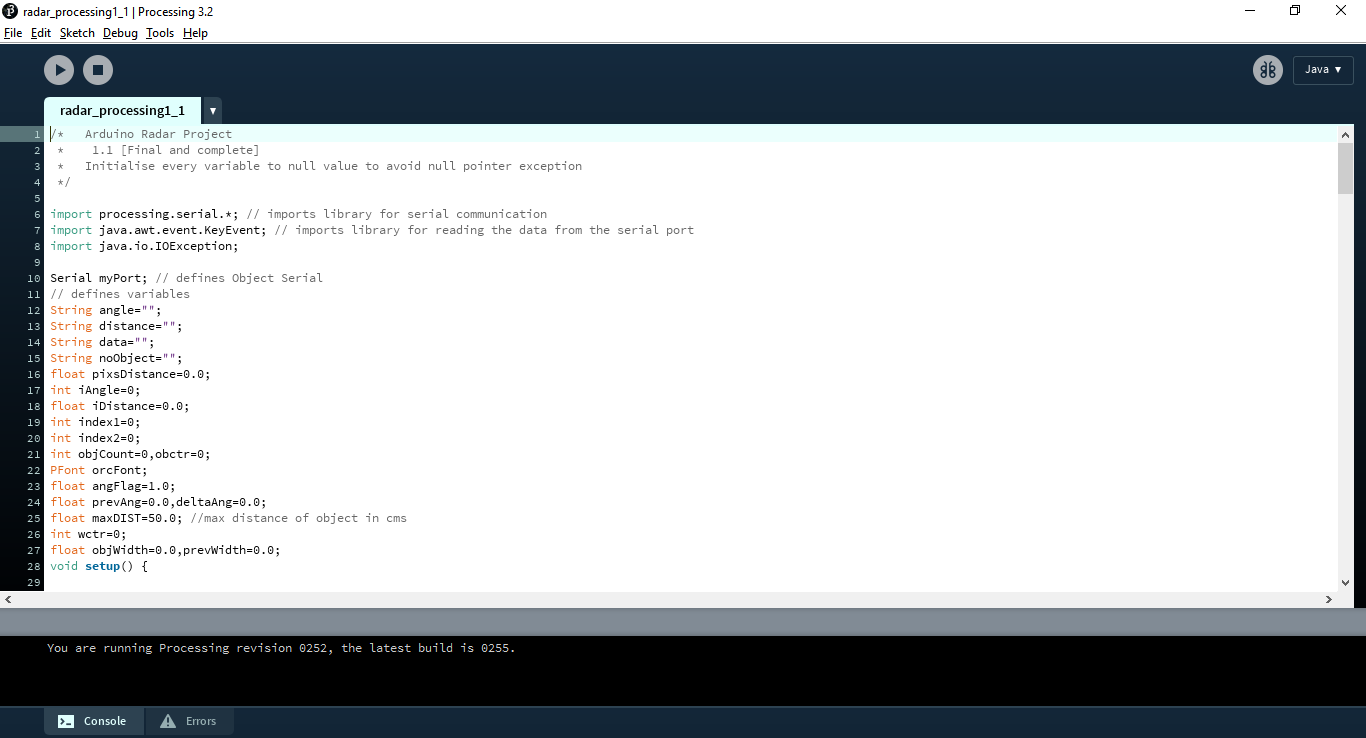
\includegraphics[width=0.7\textwidth]{../Files/processing}
	\caption{Processing}  \label{fig:processing}
\end{figure}
The code in Processing is written in \emph{Java}, and primarily consists of drawing the lines and borders of the radar map, and plotting the tracker-bar on the map. We added functionalities such as counting the number of objects, and also tried to calculate the width of the object, apart from just showing the distance of the object. \\
We made a 360 degrees map so that we could view the area according to our convenience if the angle of the set-up is changed. This angle is the "offset" that we introduced in the Arduino code. The entire Arduino and Processing codes are shown in Appendix \ref{ch:appAlabel} and Appendix \ref{ch:appBlabel}, respectively.
\begin{figure}[H]
	\vfill
	\centering
	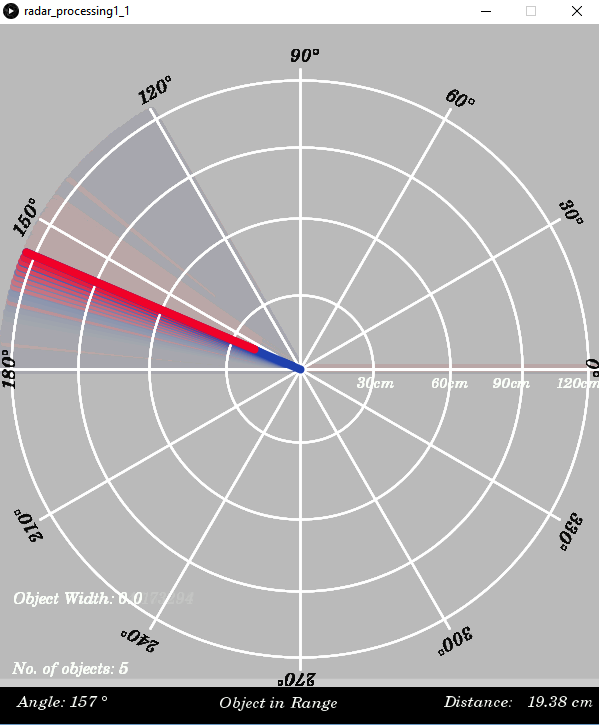
\includegraphics[width=0.7\textwidth]{../Files/radar}
	\caption{Running our code in Processing}  \label{fig:radar}
\end{figure}
\clearpage
\chapter{Explaining the Codes}
Here we'd be briefly going through the flow of the codes written for \arduino{} and in \emph{Processing}. The entire Arduino and Processing codes are given (explained with comments) in Appendix \ref{ch:appAlabel} and Appendix \ref{ch:appBlabel}, respectively.
\section{The Arduino Code}
Every \arduino{} code consists of two standard functions - \textit{void setup()} and \textit{void loop()}. The former is used to define and initialise variables, pins and the baud rate of serial communication.\\
We have programmed the Arduino to control the circuit in the following flow:
\begin{enumerate}
	\item Rotate the motor to an angle,
	\item Use the ultrasonic sensor and calculate the distance,
	\item Send both the above values via serial communication,
	\item Rotate the motor to the next degree,
	\item Repeat steps 2-5.
\end{enumerate}
The following code snippets implement the above given steps:
\begin{mdframed}[backgroundcolor=light-gray, roundcorner=10pt,leftmargin=1, rightmargin=1, innerleftmargin=15, innertopmargin=15,innerbottommargin=15, outerlinewidth=1, linecolor=light-gray]
	\begin{lstlisting}[caption={Step 1},language = C]
	// rotates the servo motor from init_ang to fin_ang degrees
	for(int i=init_ang;i<=fin_ang;i++)
	{  
	myServo.write(i-offset);  //angle value to be passed to the servo library object for writing into the motor
	delay(17);//DELAY #1:for time taken in motor rotation for one degree before calculating distance
	\end{lstlisting}
	
\begin{lstlisting}[caption={Step 2},language = C]
	distance = calculateDistance();// Calls a function for calculating the distance measured by the Ultrasonic sensor for each degree
	\end{lstlisting}
	
\begin{lstlisting}[caption={Function called above},language = C]
	// Function for calculating the distance measured by the Ultrasonic sensor
	float calculateDistance(){ 
	unsigned long T1 = micros();
	digitalWrite(trigPin, LOW); // trigPin needs a fresh LOW pulse before sending a HIGH pulse that can be detected from echoPin
	delayMicroseconds(2);//DELAY #2:time for which low trig pulse is maintained before making it high
	digitalWrite(trigPin, HIGH); 
	delayMicroseconds(10);//DELAY #3:Sets the trigPin on HIGH state for 10 micro seconds
	digitalWrite(trigPin, LOW);
	duration = pulseIn(echoPin, HIGH); // Reads the echoPin, returns the sound wave travel time in microseconds
	//distance= duration*0.034/2;
	distance = (duration/2)/29.1;     //in cm,  datasheet gives "duration/58" as the formula
	\end{lstlisting}
	
\begin{lstlisting}[caption={Step 3},language = C]
	Serial.print(i); // Sends the current degree into the Serial Port for graphical representation
	Serial.print(","); // Sends addition character right next to the previous value needed later in the Processing IDE for indexing
	Serial.print(distance); // Sends the distance value into the Serial Port for the graph
	Serial.print(";"); // Sends addition character right next to the previous value needed later in the Processing IDE for indexing
\end{lstlisting}
\end{mdframed}
\vspace{1cm}
Keeping the above code in a \texttt{void loop(){}} ensures that the steps get repeated in a loop, as desired.
\clearpage
\section{The Processing Code}
The JAVA code written for processing divides its work into a few main functions, which are customary for every code written in Processing. The functions are
\begin{itemize}
	\item \begin{verbatim}void setup()\end{verbatim} - to initialise variables and baud rate of serial communication,
	\item \begin{verbatim}void draw()\end{verbatim} - to make a 2D/3D drawing on the screen on which to show the output,
	\item \begin{verbatim}void serialEvent()\end{verbatim} - the function dealing with incoming/outgoing serial data, and operations on it.
\end{itemize}
Customised functions were used to draw several parts of the displayed graph, which were called from \texttt{void draw()}. These are :
\begin{itemize}
	\item \begin{verbatim}void drawRadar()\end{verbatim} - to draw the basic circular layer of graphics
	\item \begin{verbatim}void drawLine()\end{verbatim} - to draw a line with trails which would be used to sweep over the area implying scanning
	\item \begin{verbatim}void drawObject()\end{verbatim} - to draw a colored line over the scanning figure to indicate presence of an object, whose length would be dependant on the distance of the object from the sensor
	\item \begin{verbatim}void drawText()\end{verbatim} - to place text at different places on the map to show the serial and calculated data values
\end{itemize}
\clearpage
\chapter{Observations}
We observed data from both the serial monitor of the Arduino IDE, as well as from the graph in processing. Since we wanted our device to give the best results as quickly as possible, we decided to calibrate it.
\begin{figure}[H]
	\vfill
	\centering
	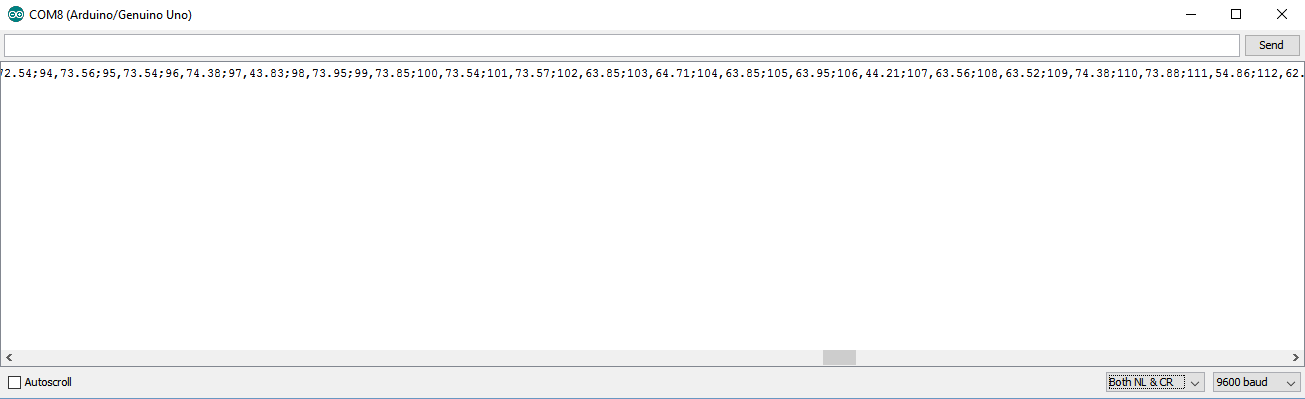
\includegraphics[width=0.7\textwidth]{../Files/sermon}
	\caption{Data Observed in the Serial Monitor of the Arduino IDE}  \label{fig:sermon}
\end{figure}
\section{Calibration}
\subsection{Calibration of Measurements}
We realised that actual measurements of distance/count/width of an object placed in the vicinity of the apparatus were different from the ones provided by our device. Hence, we proceeded to calibrate each part of our device that was capable of taking a measurement.\\

The quantities that were measured in our project before going for any further calculations were: \underline{Angle} and \underline{Distance}. The rest were only obtained by playing around with these two main quantities. Hence, we needed them to be as accurate as possible.\\

We did not notice any error in the value of angle that the motor was rotating to, hence we did not have to do any sort of calibration for it.\\

To calibrate the distance, we placed several objects at fixed distances from the sensor on a white chart paper, with values of distances marked on it with the help of a ruler. We then made measurements keeping the sensor still, and made an adjustment to the formula in the code by observing the multiplication factor that needed to be introduced into the previous formula in order to get the correct values. Hence, the formula was changed from "duration/58" to "duration/58.2".\\
\begin{figure}[H]
	\vfill
	\centering
	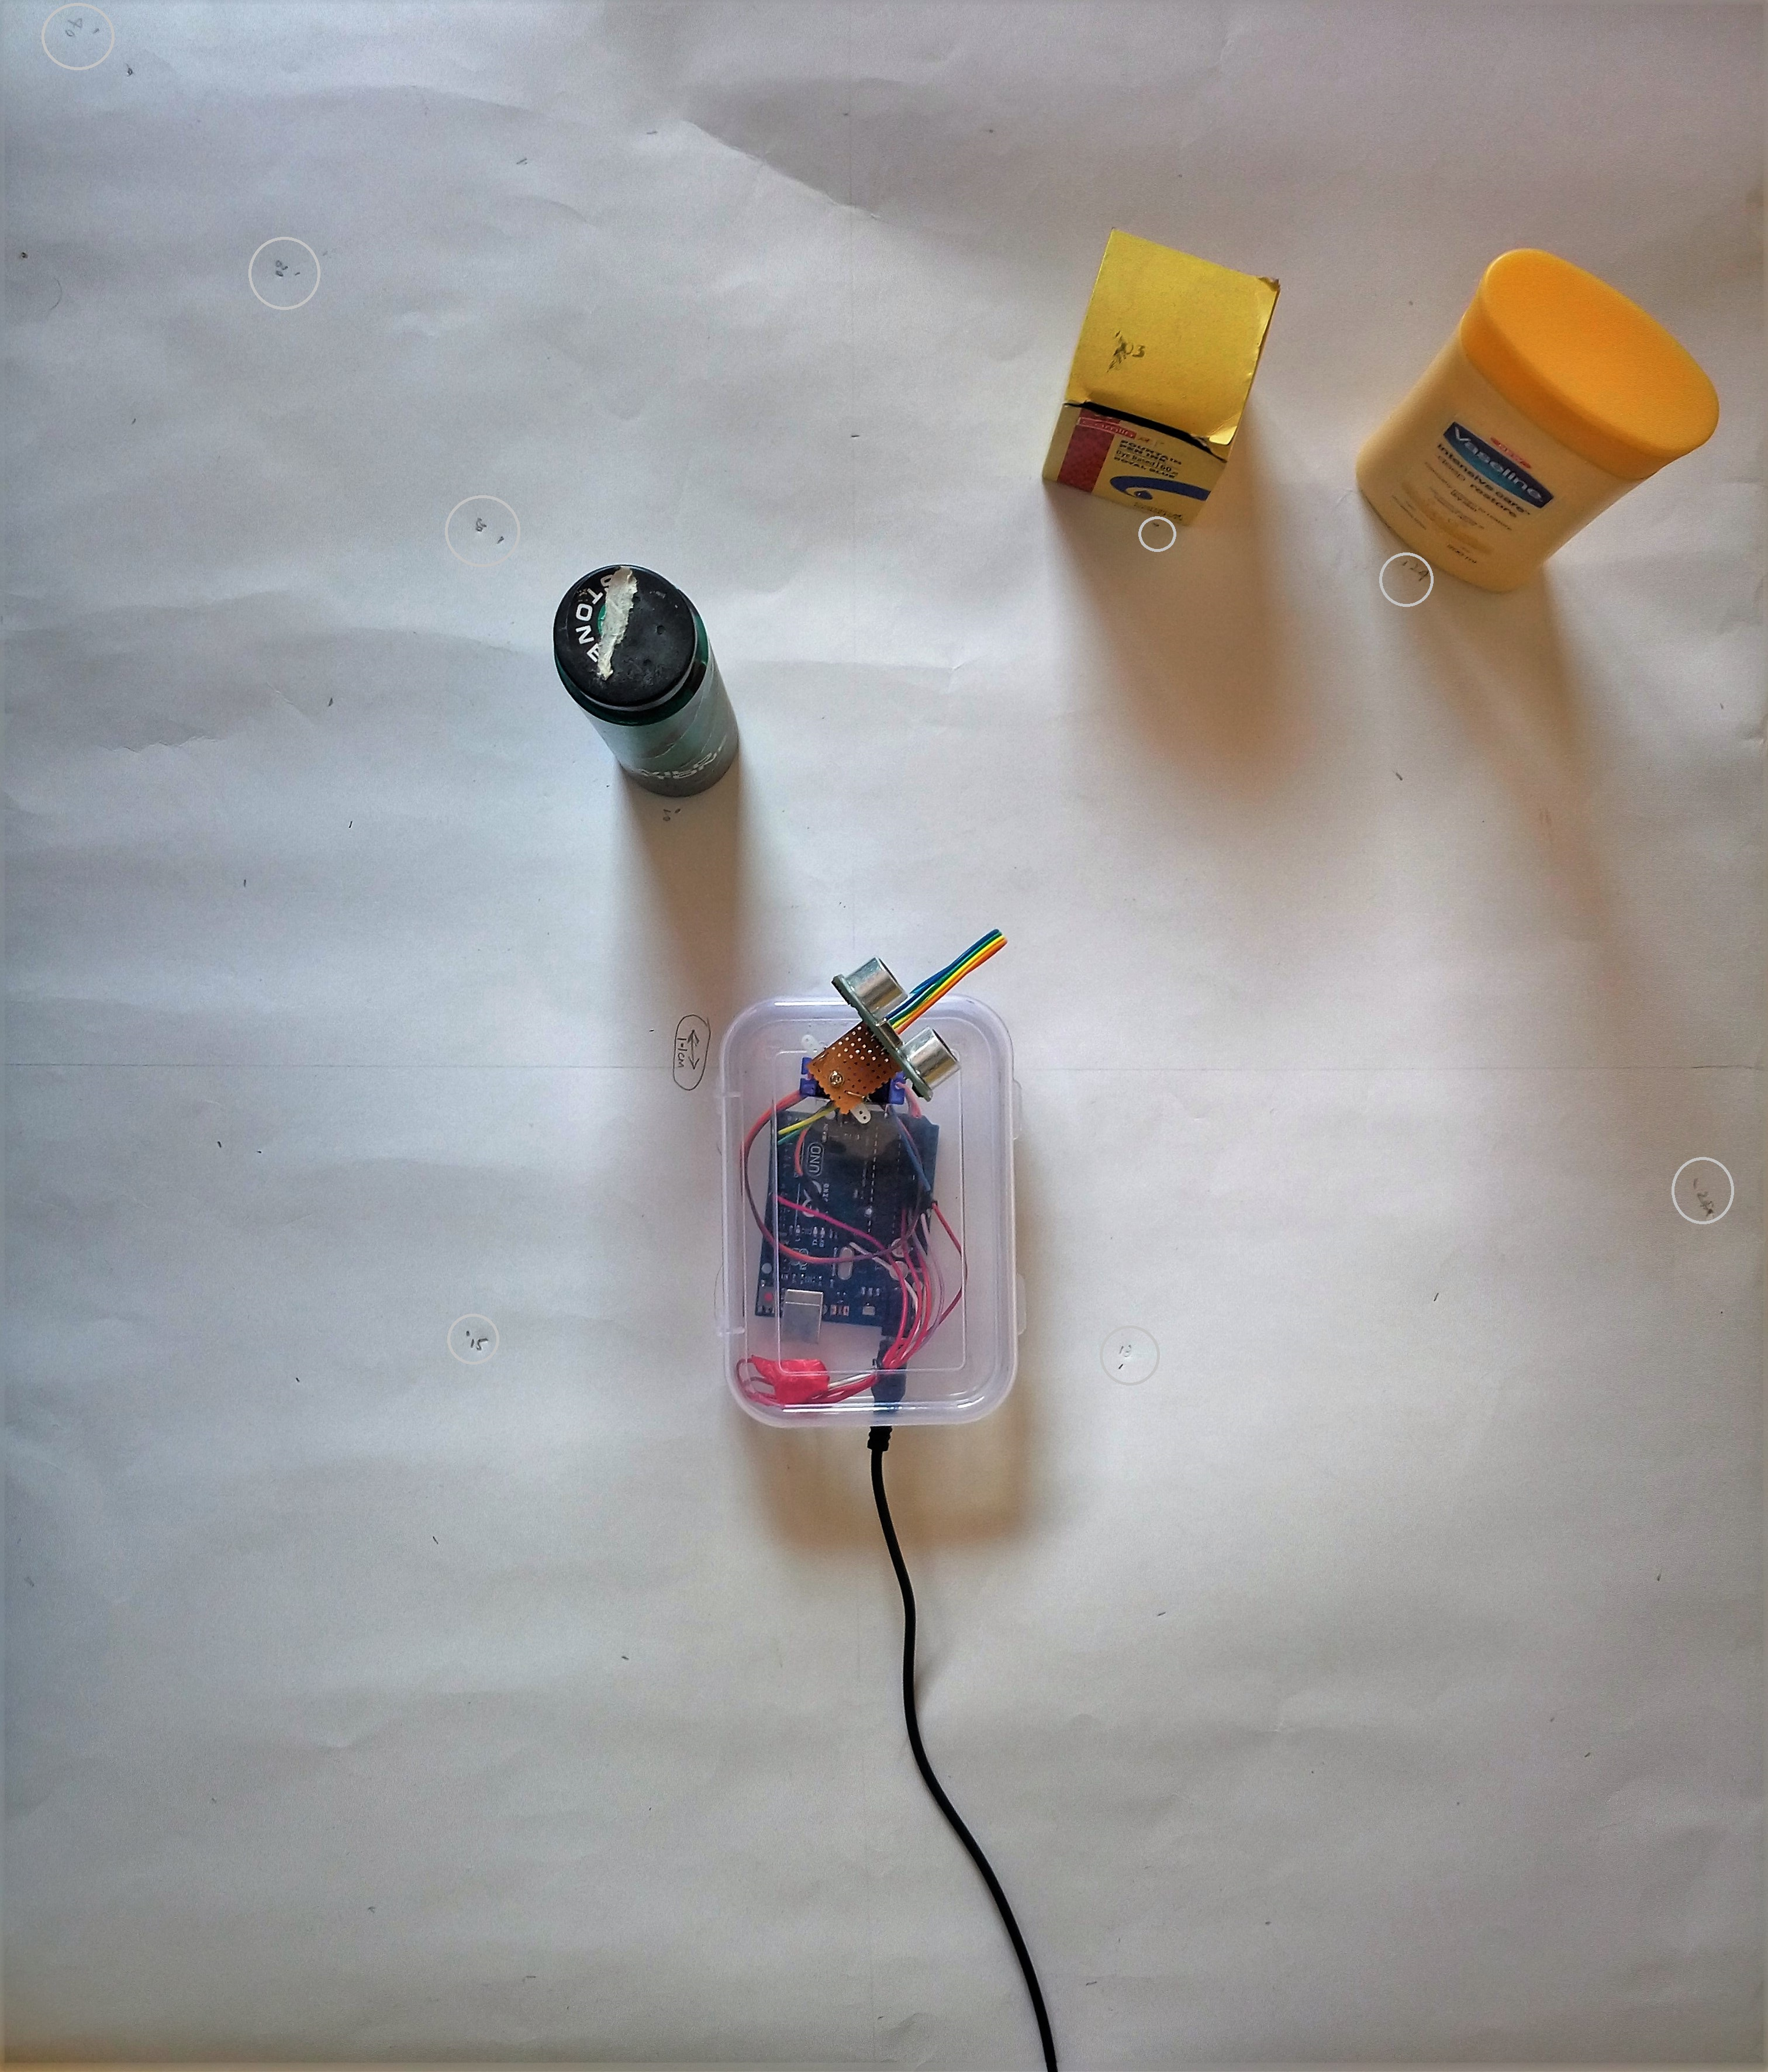
\includegraphics[width=\textwidth]{../Files/cabri.jpg}
	\caption{Calibration on chart paper with marked distances}  \label{fig:sermon}
\end{figure}
\subsection{Optimising Speed}
We wanted to optimise our device to work as quickly as possible, without affecting normal execution of the program. So we optimised our code, considering the delays in physical movement, time periods of recieved/transmitted waves and time taken to process the data.\\
We took into account the several delays introduced in the code, along with the delay in rotation of the motor(specified by its speed given in its datasheet, tested to be accurate) and delay in calculation of distance. Accordingly, we minimised each of the values given as arguments to the \begin{verbatim}delay()\end{verbatim} function used at different parts of the Arduino code, to the safest least value possible. Each of the delays with descriptions can be observed in the Arduino code given with comments in Appendix \ref{ch:appAlabel}
\section{Graphs}
We obtained the following [error vs. position] graphs for three different kinds of objects kept in front of the sensor. In each case, we noted down values for both the sensor being stationary, and rotating. The three different kinds of objects were
\begin{itemize}
	\item Object1 = Hollow plastic bottle (width=6cm)
	\item Object2 = Solid DC battery (width=3cm)
	\item Object3 = Metallic pen (width=0.8cm)
\end{itemize}

\begin{figure}[H]
	\vfill
	\centering
	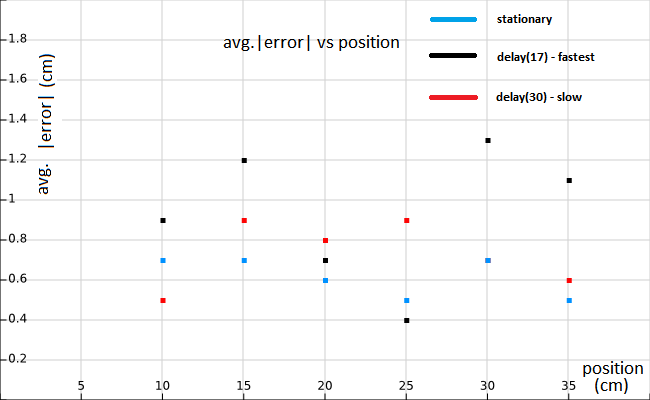
\includegraphics[width=0.8\textwidth]{../Files/save12}
	\caption{Object1-avg.|error| vs position} 
\end{figure}
\begin{figure}[H]
	\vfill
	\centering
	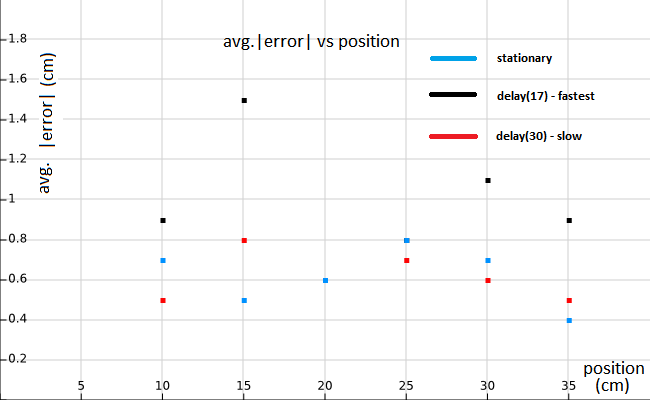
\includegraphics[width=0.8\textwidth]{../Files/save21}
	\caption{Object2-avg.|error| vs position} 
\end{figure}
\begin{figure}[H]
	\vfill
	\centering
	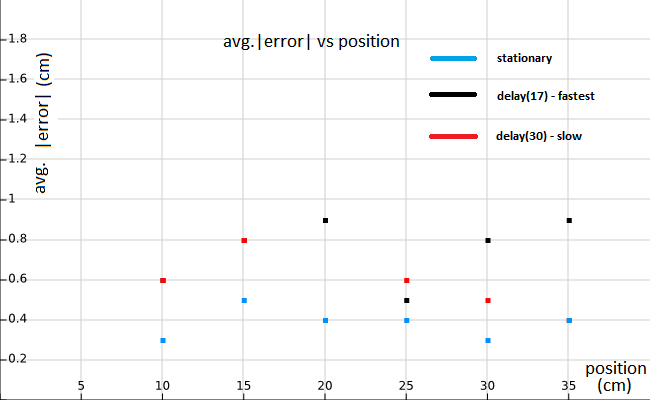
\includegraphics[width=0.8\textwidth]{../Files/save32}
	\caption{Object3-avg.|error| vs position}  
\end{figure}
\clearpage
Finally, we also plotted the error in data of width of object vs. position, which was something like this:
\begin{figure}[H]
	\vfill
	\centering
	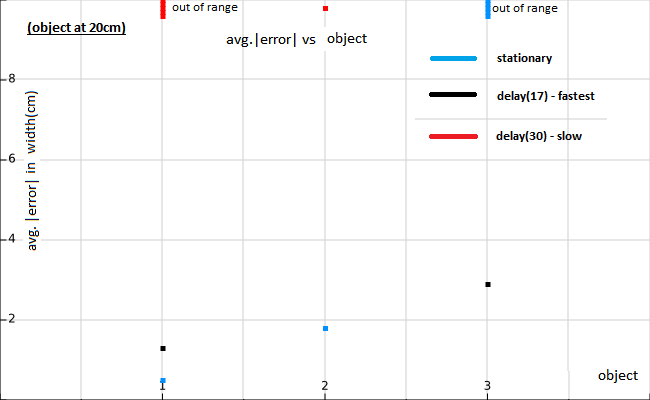
\includegraphics[width=\textwidth]{../Files/savew1}
	\caption{Object-wise avg.|error| in width at x=20cm} 
\end{figure}
\clearpage
\section{Challenges}
As observed from the graphs plotted in the previous section, we are not able to determine any particular increasing/decreasing order being followed by the errors in measurement of the "distance" quantity. Moreover, by increasing the speed of measurement of the device (by reducing the manual delays introduced inside the Arduino code within safe limits), the error does not necessarily seem to increase with speed. The "width of the object" quantity seems to be correct at one instant and completely wrong at any other instant with very random error values.\\
However, what we did observe were sudden jumps in errors. Among several trials, their occurrence increased with the speed. That is, the device was detecting \textit{stray} values, and the amount of stray values per experiment increased with the speed of the device. 
\section{Identified Problem}
With the help of ideas from several online electronics forums, we carefully studied the flow of the code, which exposed the flaw in our logic. The problem lied in the fact that the code took variable amount of time in calculating the distance of an object, proportional to the distance itself. This fact could be derived from the line in the code\begin{verbatim}duration = pulseIn(echoPin, HIGH);\end{verbatim} where the function pulseIn starts a counter which counts till the value at echoPin is HIGH.\\
Here, our program only waited to recieve the first returning pulse, before quickly sending the output and turning the motor to the next angle. At some instances, this could mean that by the time the sensor was ready to take a new measurement, the older echo pulses were still arriving at the receiver, hence a wrong measurement. The older echo pulses could still be around due to \\
(a) The program having quickly moved to the next set of commands and having made the sensor ready to receive ultrasonic waves - this, within the time in which the remaining of the 8 pulses were still being recieved at the reciever, or \\
(b) Due to the waves being spherical in nature and the field of view of the sensor being 15 degrees, the waves could've been reflected by some undesired obstacles in the field of view. It could also be the result of multiple reflections.
\section{Proposed Solution}
Therefore, we edited the algorithm in such a way, that between each degree of rotation of the motor, the program takes the exact amount of time to run. That is, the program makes up for the time left out compared to the extreme-time-taking case by waiting.\\
We did this by using the fact to our advantage that the maximum time taken by the calculateDistance() function is when there is no obstacle. The \hcsr{} sensor waits for 38ms in case no object is detected, before giving a HIGH echo signal. Hence, we ensure that the program always takes a total of 38ms for each iteration of the loop. For this, we used the \emph{micros()} function inside the \textit{calculateDistance()} function of the arduino code, which calculates the number of microseconds elapsed till the code execution started.\\
Here's the added portion of code which did our solution:
\begin{mdframed}[backgroundcolor=light-gray, roundcorner=10pt,leftmargin=1, rightmargin=1, innerleftmargin=15, innertopmargin=15,innerbottommargin=15, outerlinewidth=1, linecolor=light-gray]
	\begin{lstlisting}[caption={Corrected calculateDistance() function},language = C]
	// Function for calculating the distance measured by the Ultrasonic sensor
	float calculateDistance(){ 
	unsigned long T1 = micros();
	digitalWrite(trigPin, LOW); // trigPin needs a fresh LOW pulse before sending a HIGH pulse that can be detected from echoPin
	delayMicroseconds(2);//DELAY #2:time for which low trig pulse is maintained before making it high
	digitalWrite(trigPin, HIGH); 
	delayMicroseconds(10);//DELAY #3:Sets the trigPin on HIGH state for 10 micro seconds
	digitalWrite(trigPin, LOW);
	duration = pulseIn(echoPin, HIGH); // Reads the echoPin, returns the sound wave travel time in microseconds
	//distance= duration*0.034/2;
	distance = (duration/2)/29.1;     //in cm,  datasheet gives "duration/58" as the formula
	
	//To avoid sending data at variable time intervals due to varying time duration taken between execution of above code inside this function depending on distance of obstacle
	//if no object, echo pulse is HIGH after 38ms
	while(micros()-T1<38000)
	{
	;
	}
	
	return distance;
	}
	\end{lstlisting}
	\end{mdframed}
	\clearpage
Here are the graphs replotted for the data obtained after correction
	\begin{figure}[H]
		\vfill
		\centering
		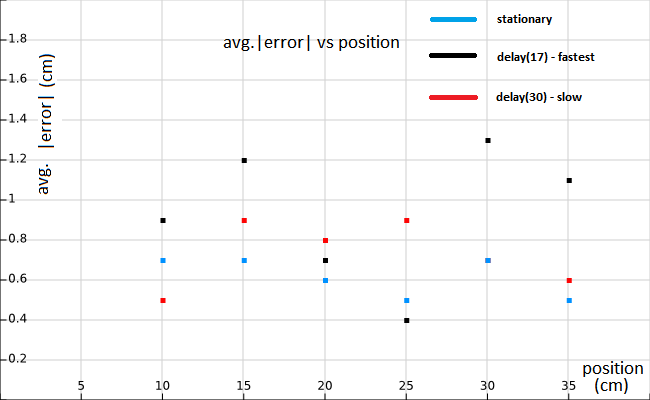
\includegraphics[width=0.8\textwidth]{../Files/save12}\\
		
		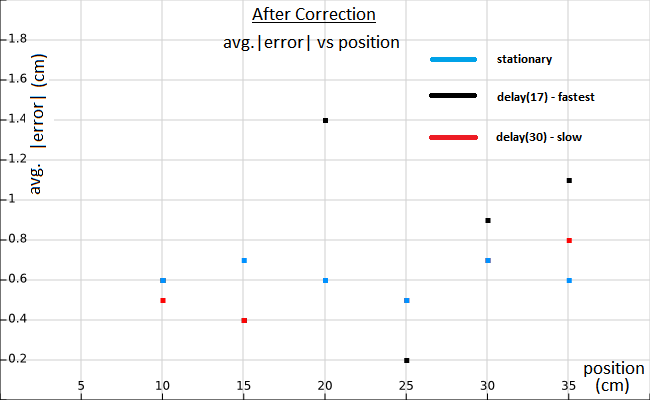
\includegraphics[width=0.8\textwidth]{../Files/save11}
		\caption{Object1-avg.|error| vs position, before vs. after correction}  
	\end{figure}
	\begin{figure}[H]
		\vfill
		\centering
		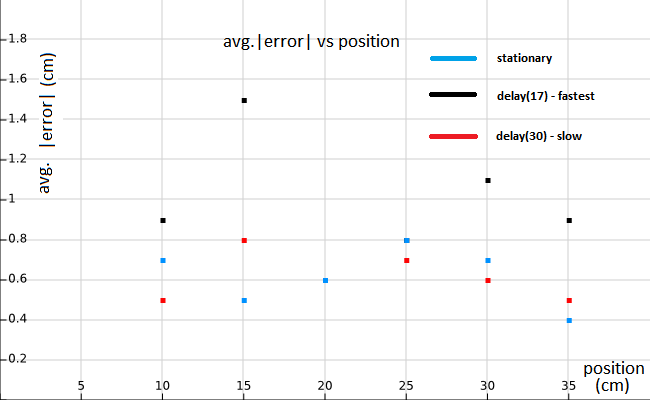
\includegraphics[width=0.8\textwidth]{../Files/save21}\\
		
		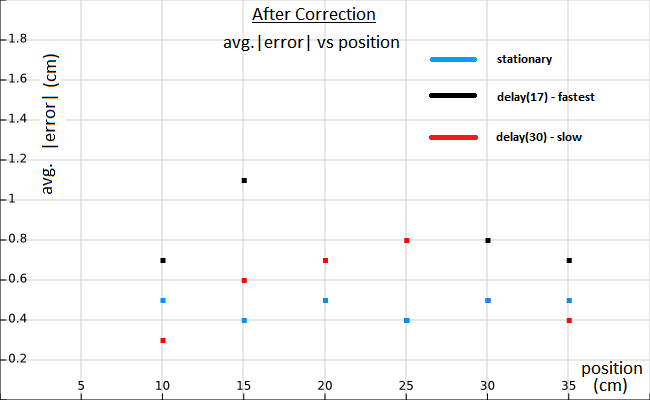
\includegraphics[width=0.8\textwidth]{../Files/save20}
		\caption{Object2-avg.|error| vs position, before vs. after correction}  
	\end{figure}
	\begin{figure}[H]
		\vfill
		\centering
		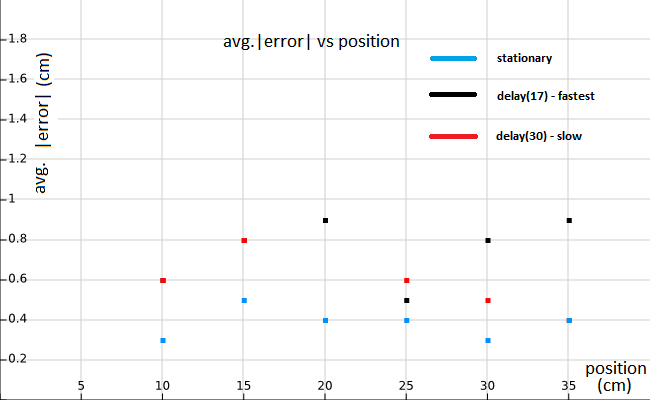
\includegraphics[width=0.8\textwidth]{../Files/save32}\\
		
		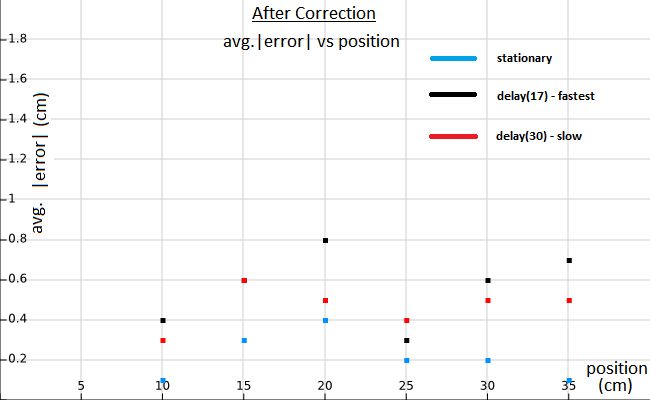
\includegraphics[width=0.8\textwidth]{../Files/save31}
		\caption{Object3-avg.|error| vs position, before vs. after correction}  
	\end{figure}
	\begin{figure}[H]
		\vfill
		\centering
		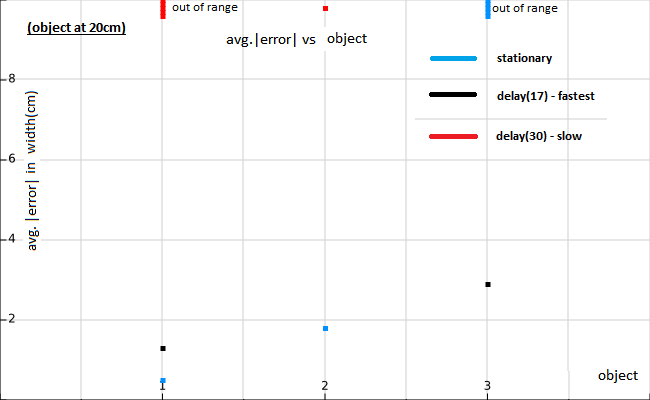
\includegraphics[width=0.8\textwidth]{../Files/savew1}\\
		
		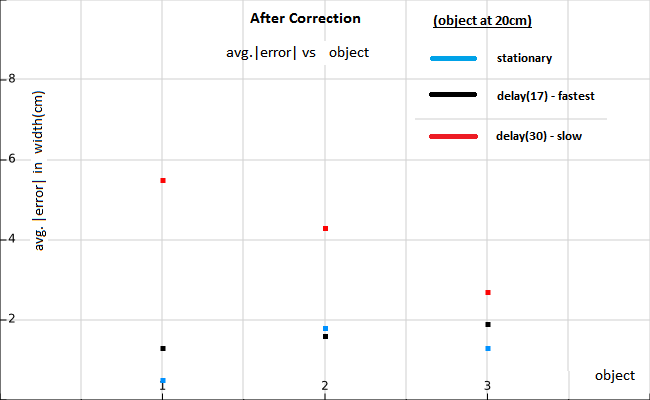
\includegraphics[width=0.8\textwidth]{../Files/savew2}
		\caption{Object-wise:avg.|error| in width at x=20cm, before vs. after correction}  
	\end{figure}

\chapter{Conclusion}

<Conclusion here>

%\chapter{The Team}
\begin{figure}[H]
	\vfill
	\centering
	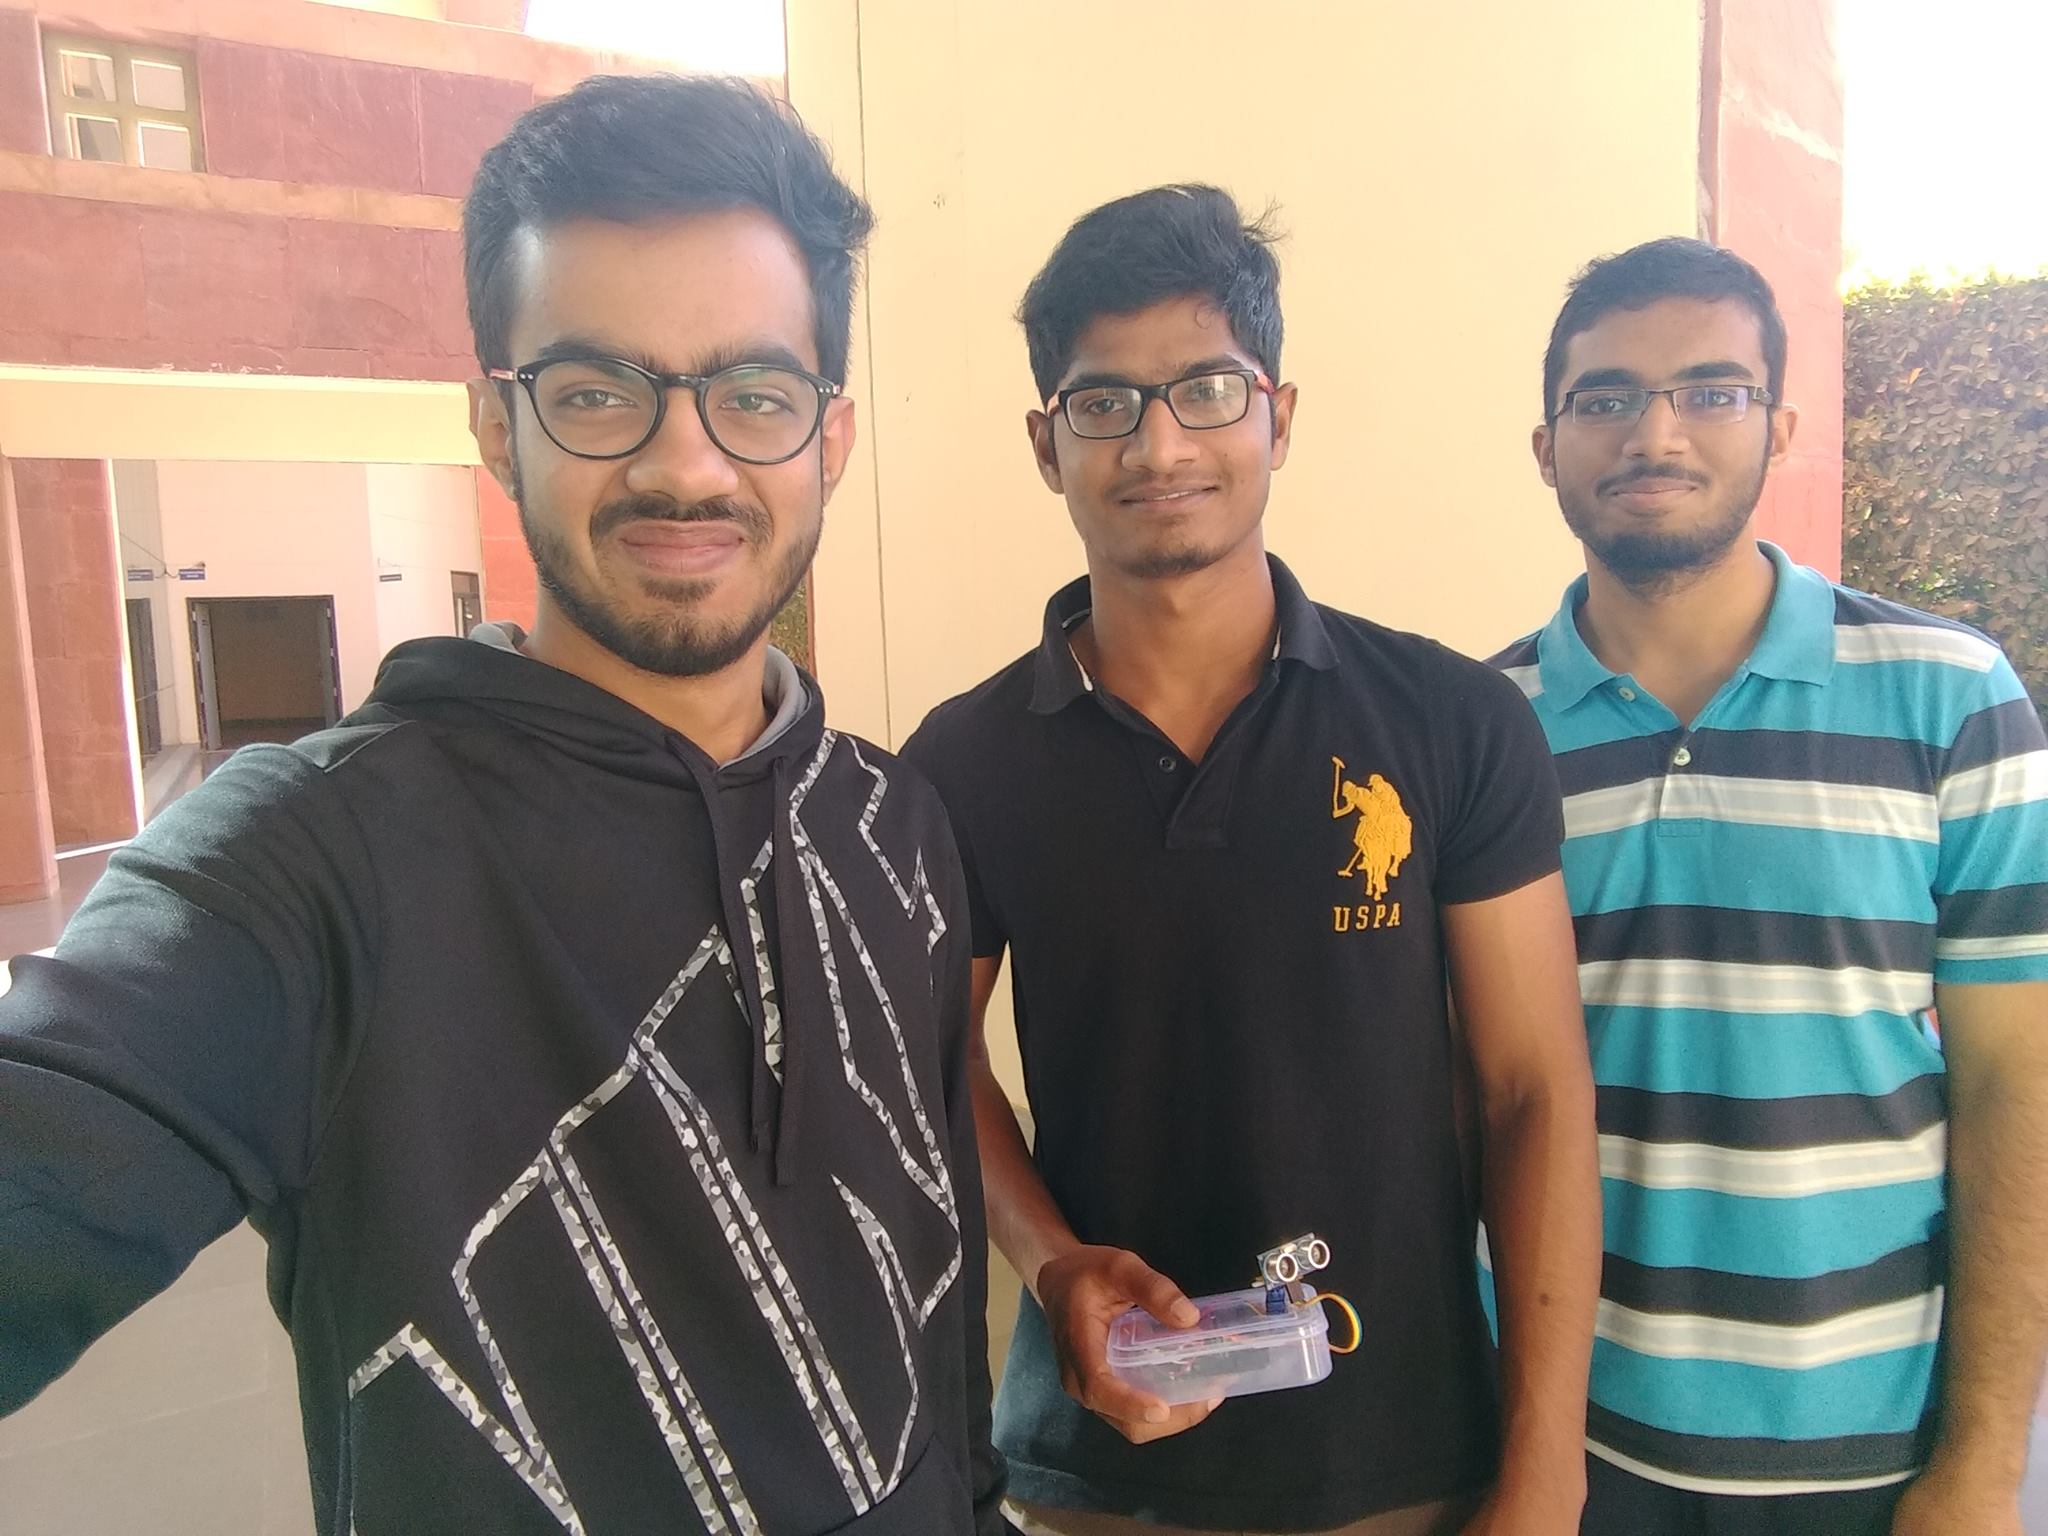
\includegraphics[width=0.5\textwidth]{../Files/team.jpg}
	\caption{The Team : From Left to Right - Sumit, Nikhil and Surya}  \label{fig:team}
\end{figure}
\begin{figure}[H]
	\vfill
	\centering
	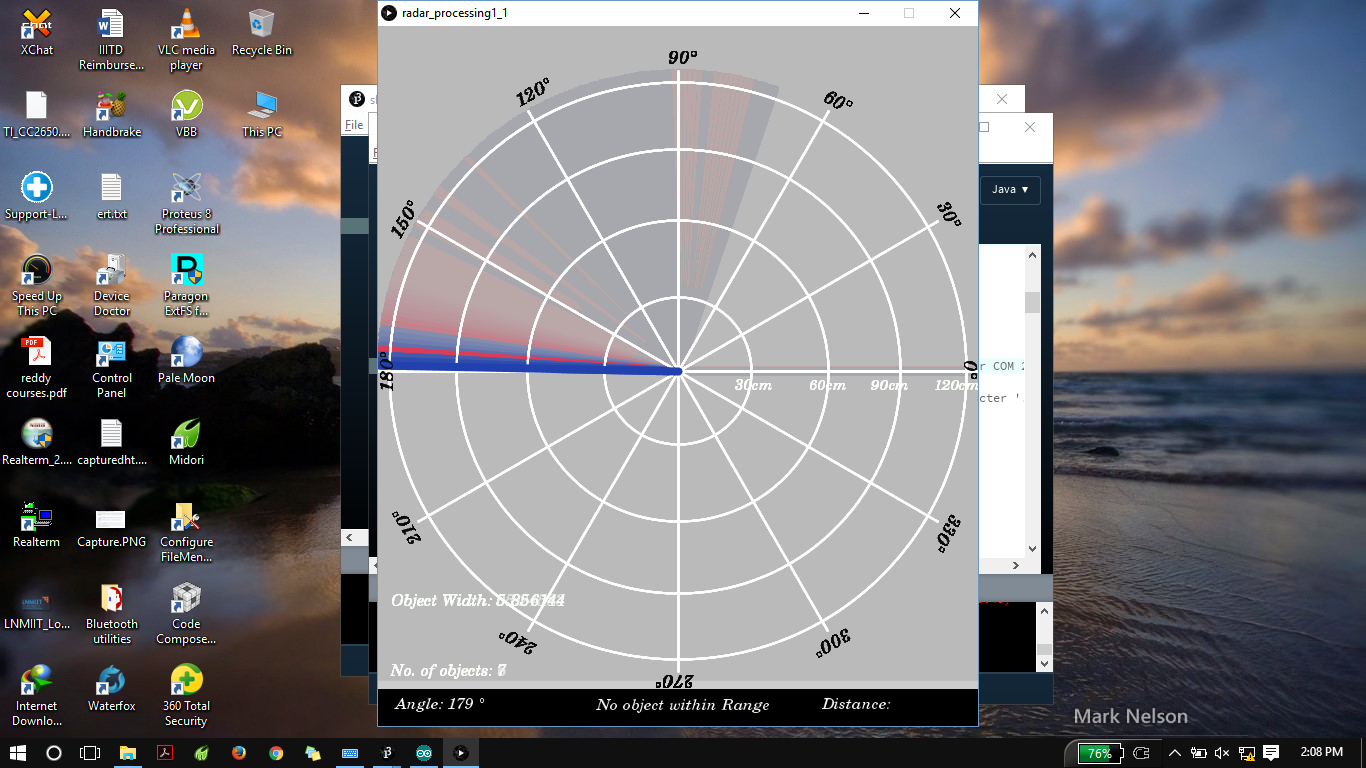
\includegraphics[width=0.4\textwidth]{../Files/project}
	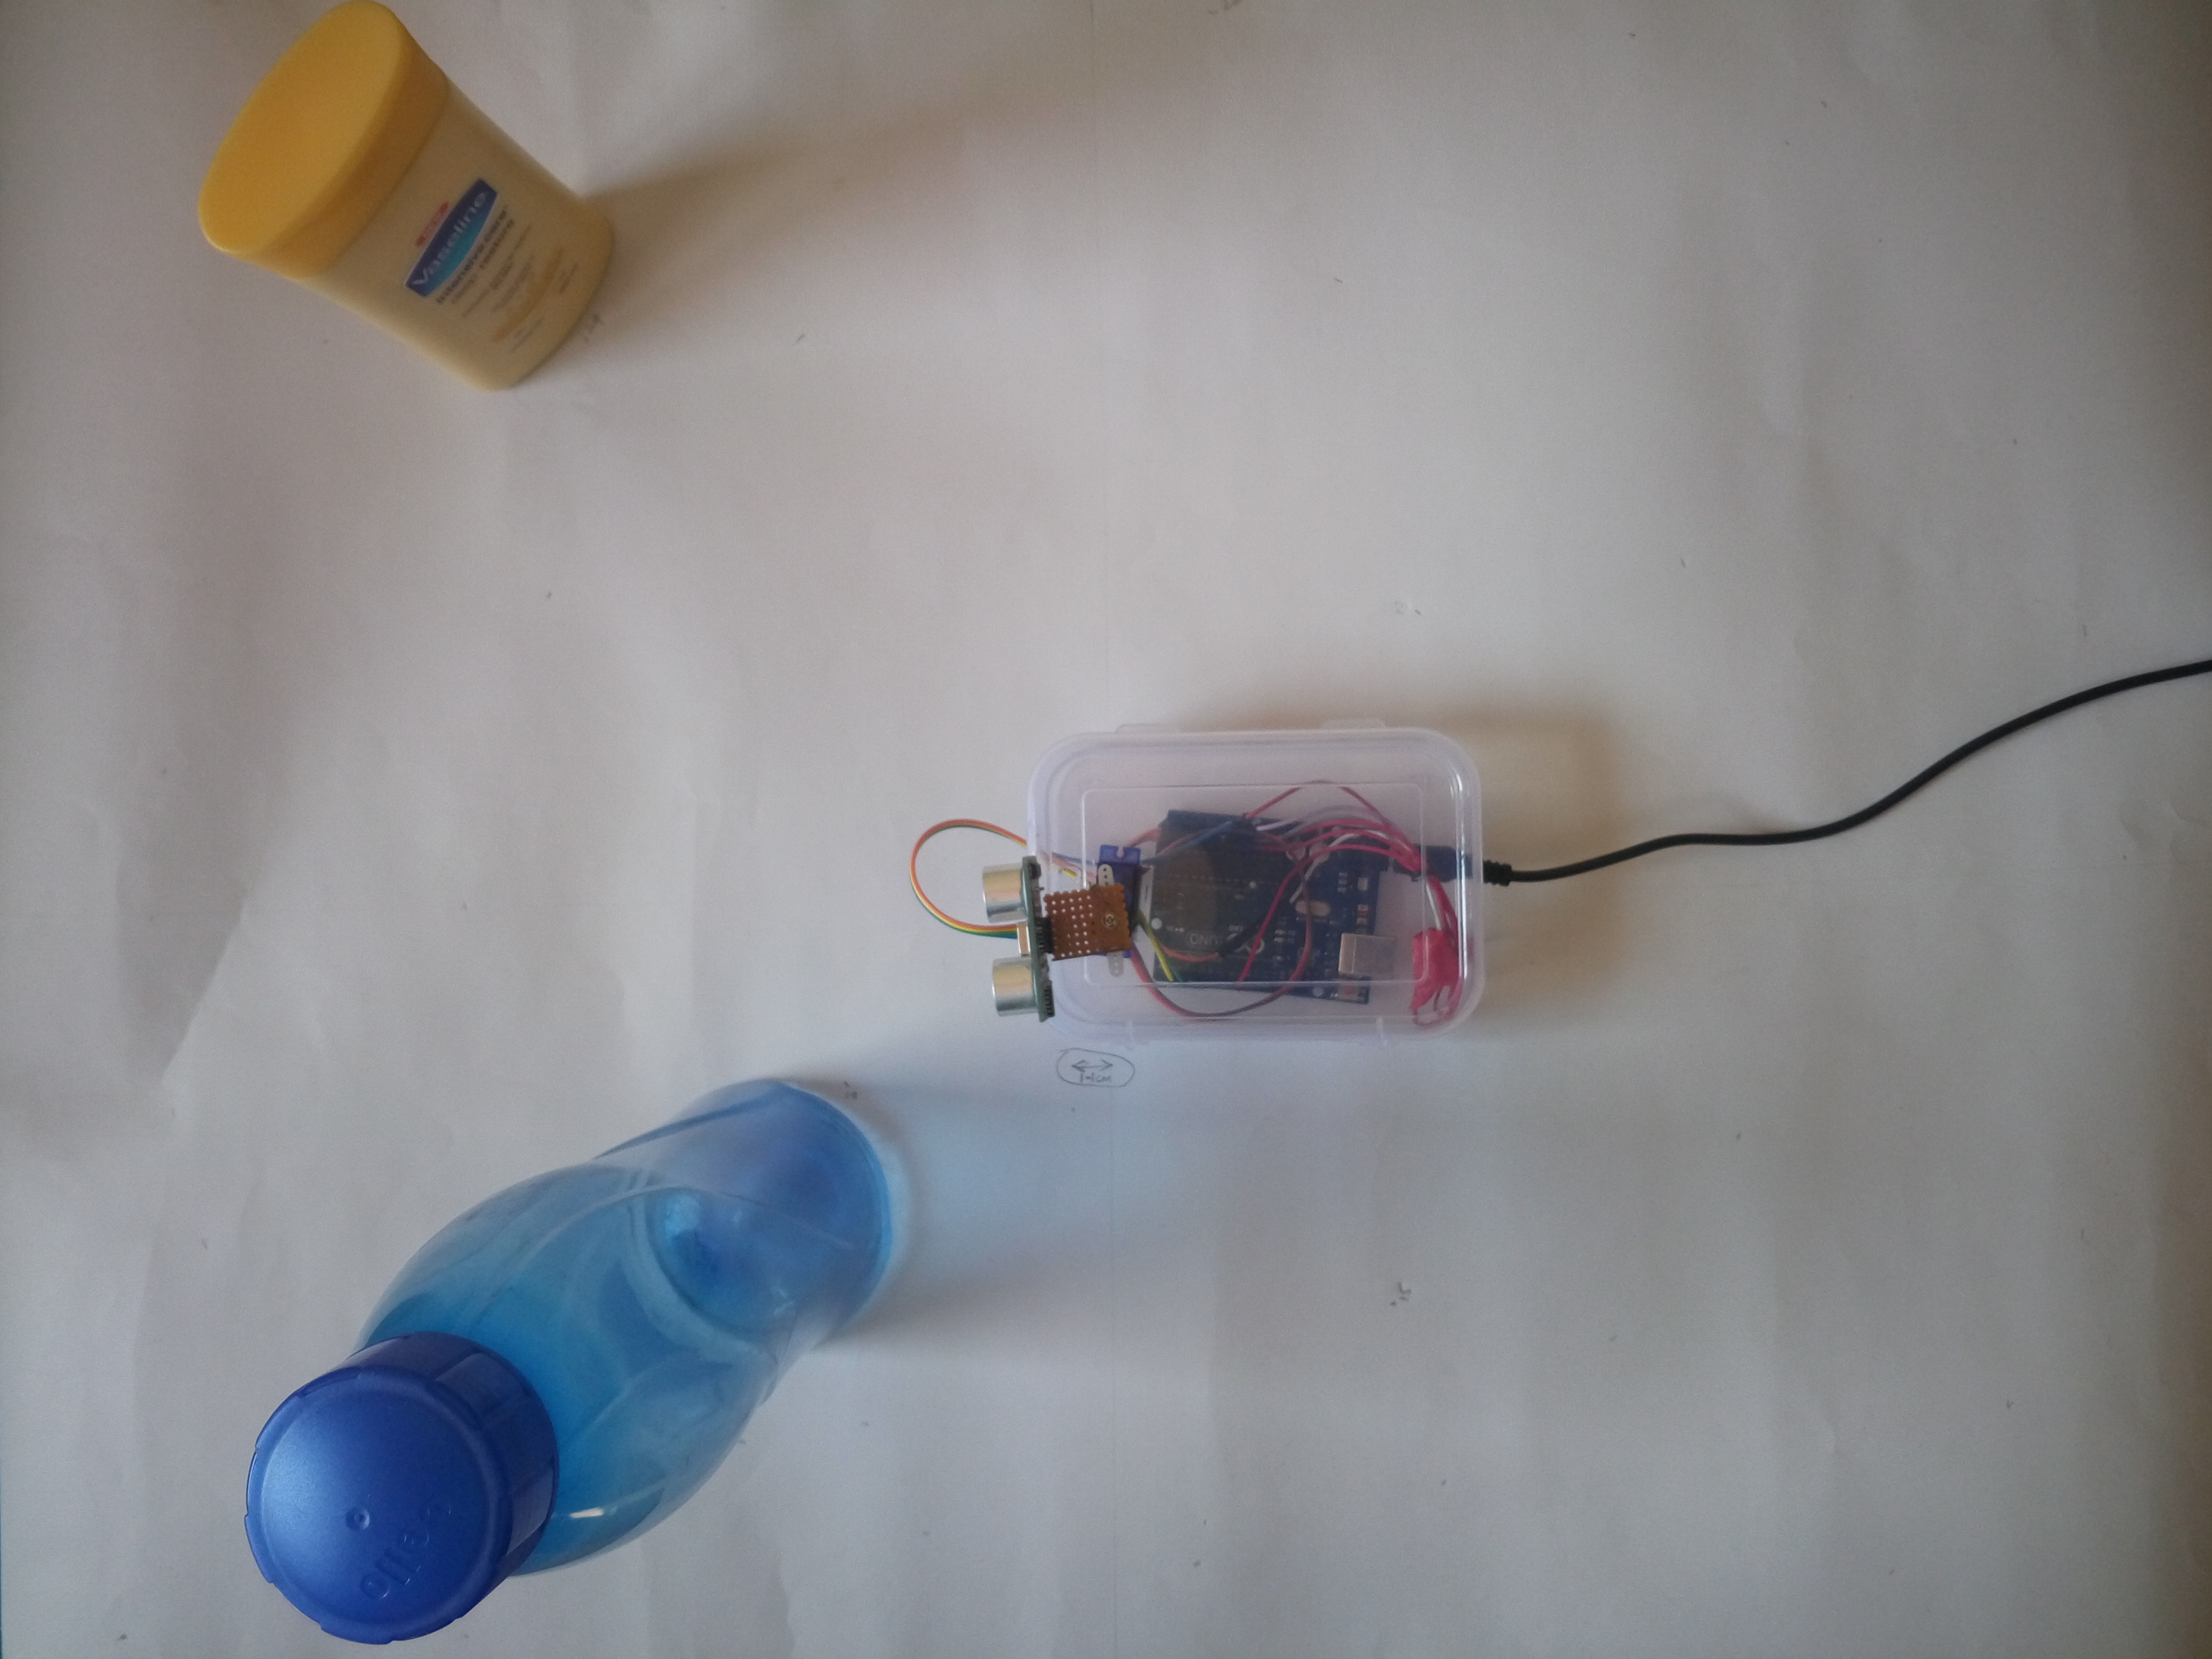
\includegraphics[width=0.4\textwidth]{../Files/project2.jpg}
	\caption{The project}  \label{fig:pro}
\end{figure}
%\printbibliography[heading=bibintoc]
%\label{bib:mybiblio}
\appendix
\chapter{Acknowledgements}
We are deeply grateful to our teacher, mentor and team leader; Dr. Deepak Nair, who held us through the course of the semester and made us learn things in a very systematic way. This in itself was solely responsible for teaching us with deep practice, new skills and methods which could have been easily missed out, otherwise. \vspace{1cm}

Thanks to sir's guidance, not a single portion of the project, however rudimentary it could've sounded, was devoid of new knowledge and appropriate professional methodology. \vspace{1cm}

We'd like to thank our institute, the LNMIIT Jaipur, for having granted us the resources,freedom and opportunity to embark on a project of our choice, which has taught us so much. \clearpage
\chapter{The Team}
\begin{figure}[H]
	\vfill
	\centering
	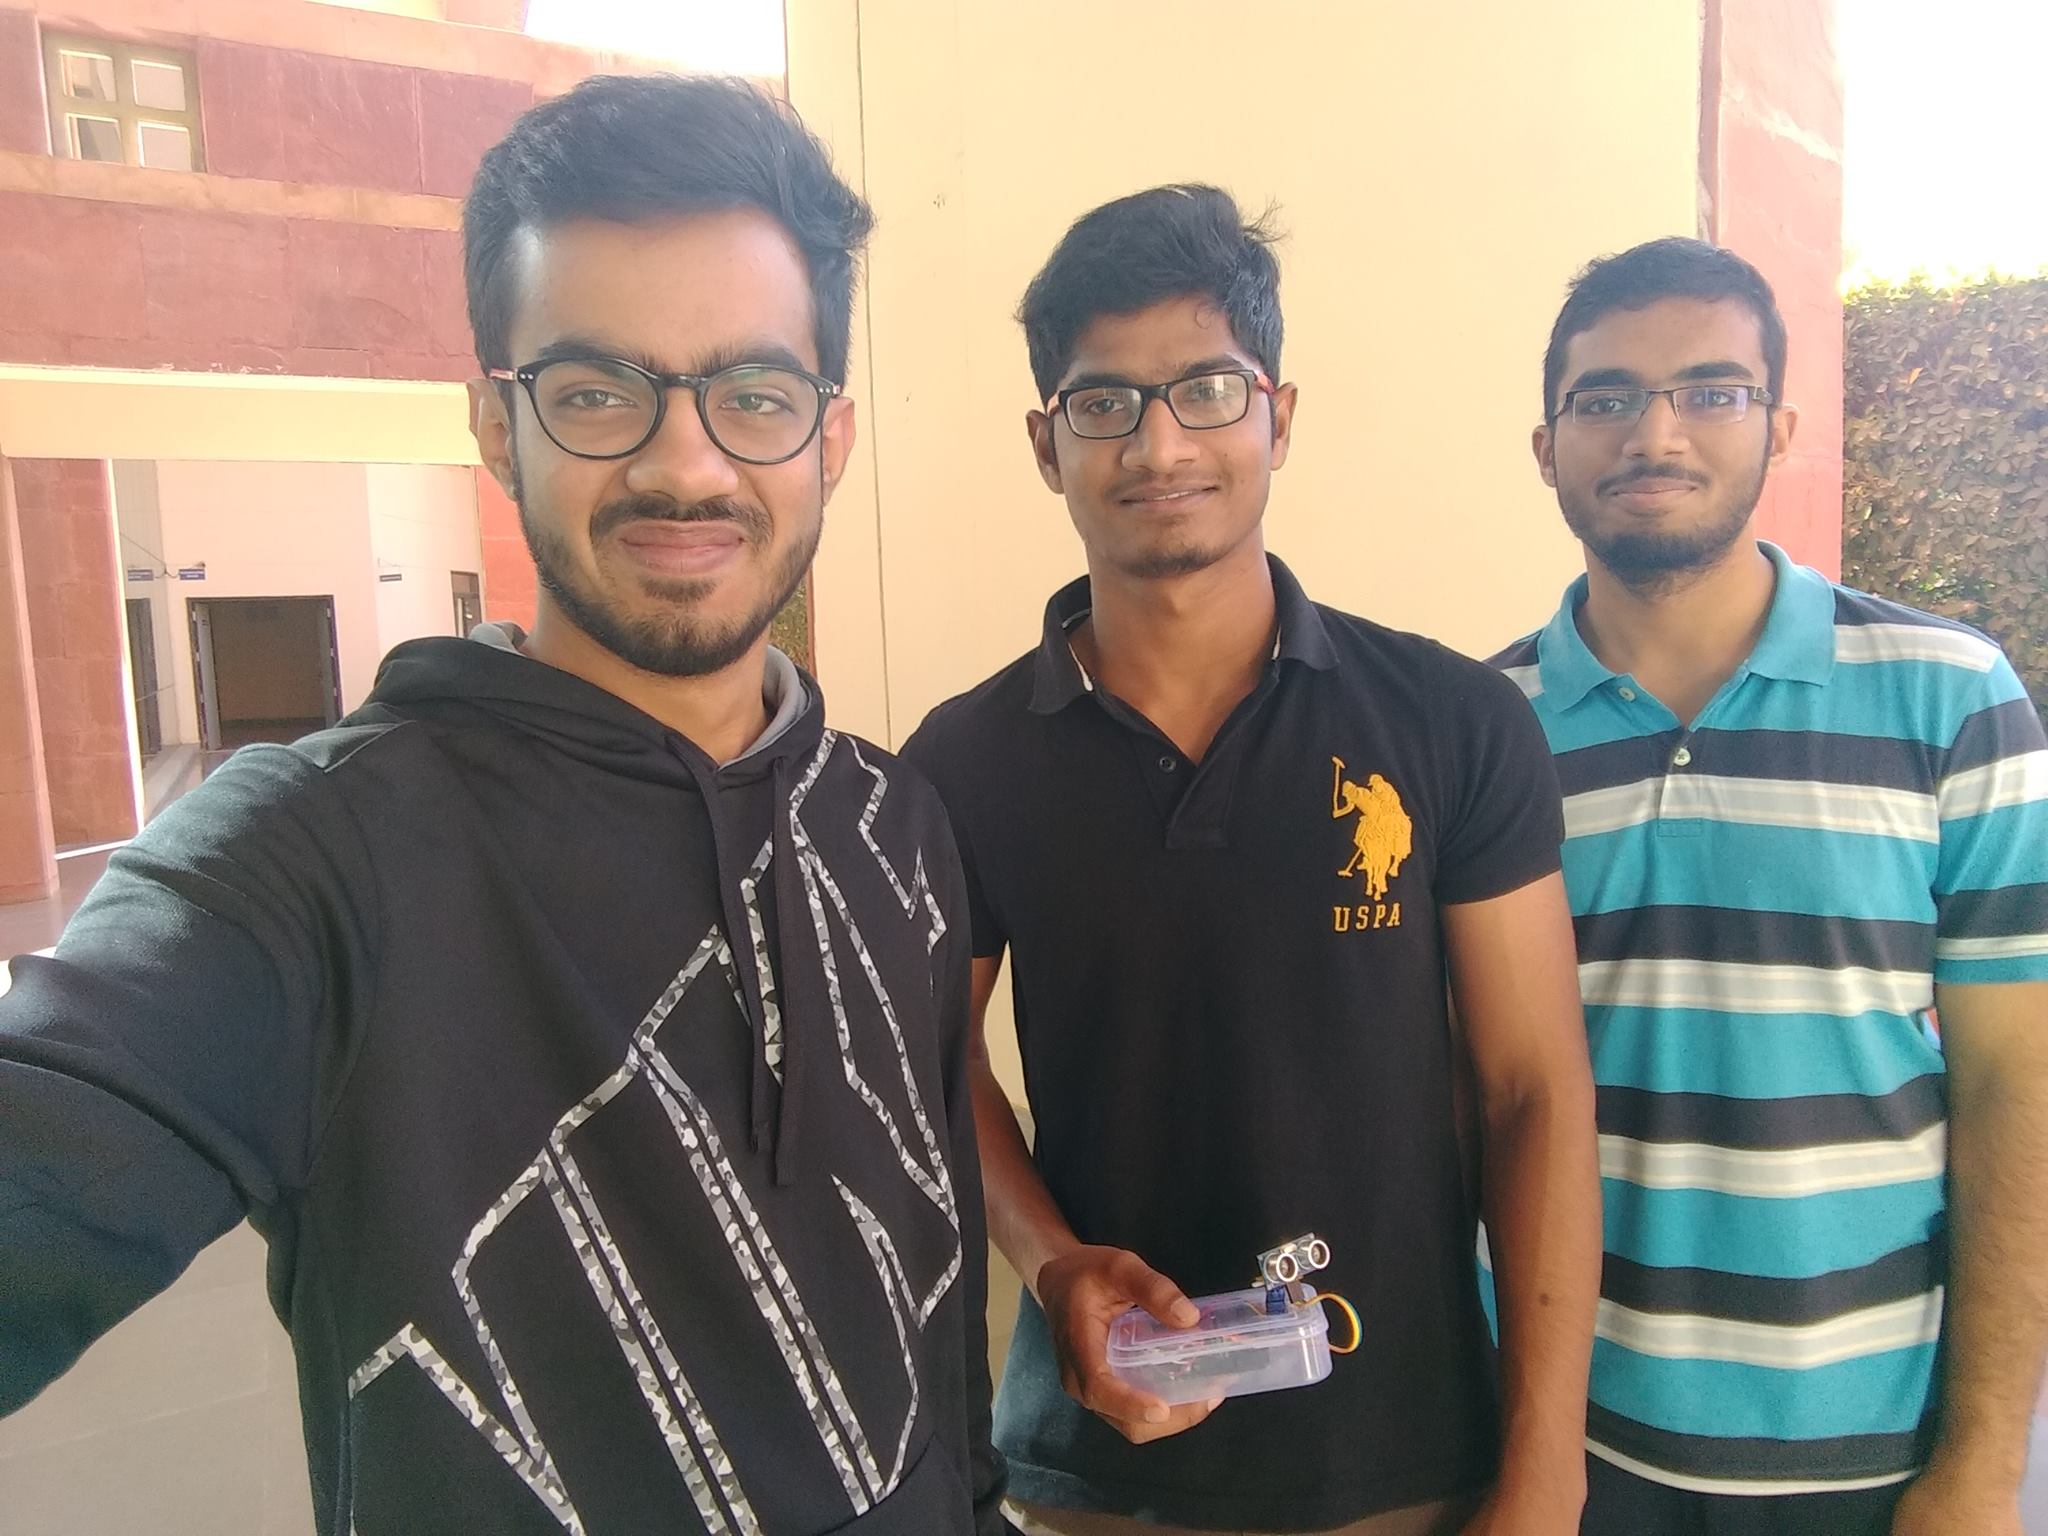
\includegraphics[width=0.5\textwidth]{../Files/team.jpg}
	\caption{The Team : From Left to Right - Sumit, Nikhil and Surya}  \label{fig:team}
\end{figure}
\begin{figure}[H]
	\vfill
	\centering
	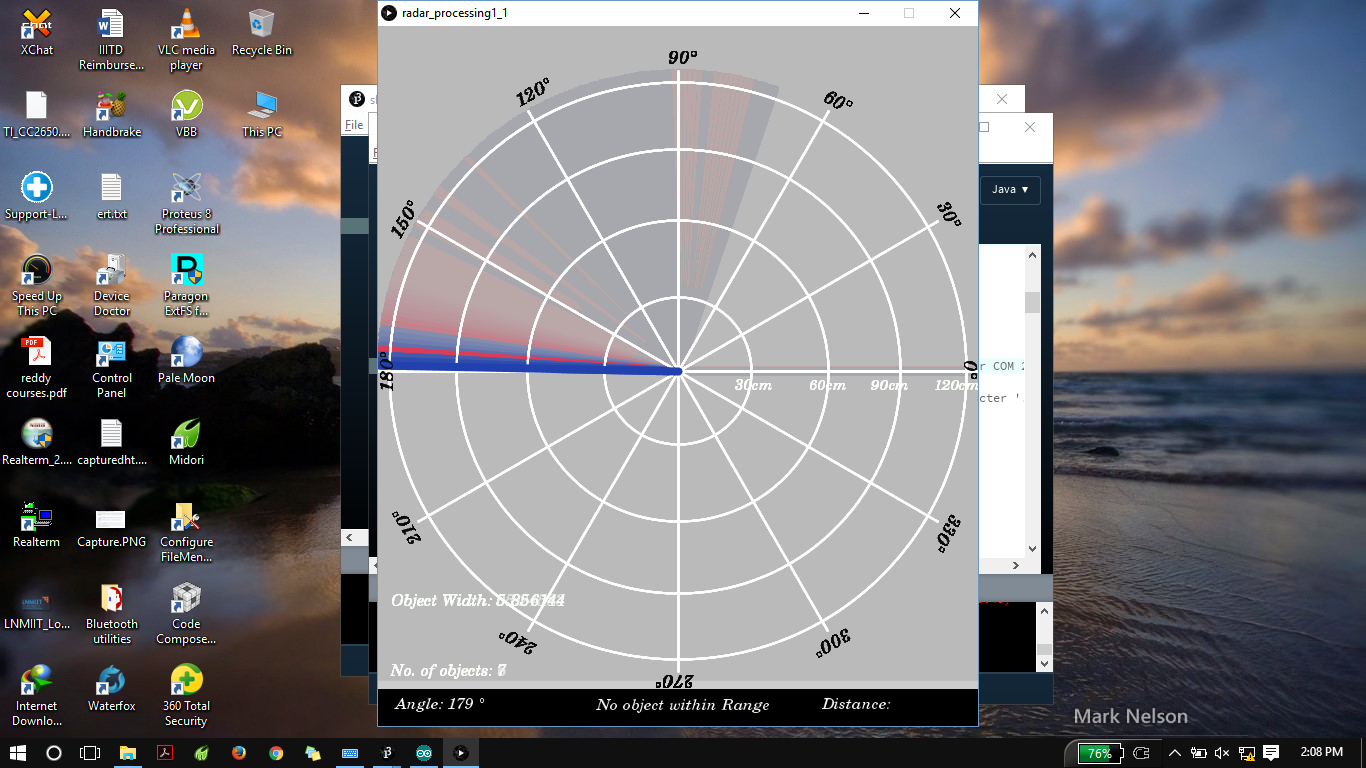
\includegraphics[width=0.4\textwidth]{../Files/project}
	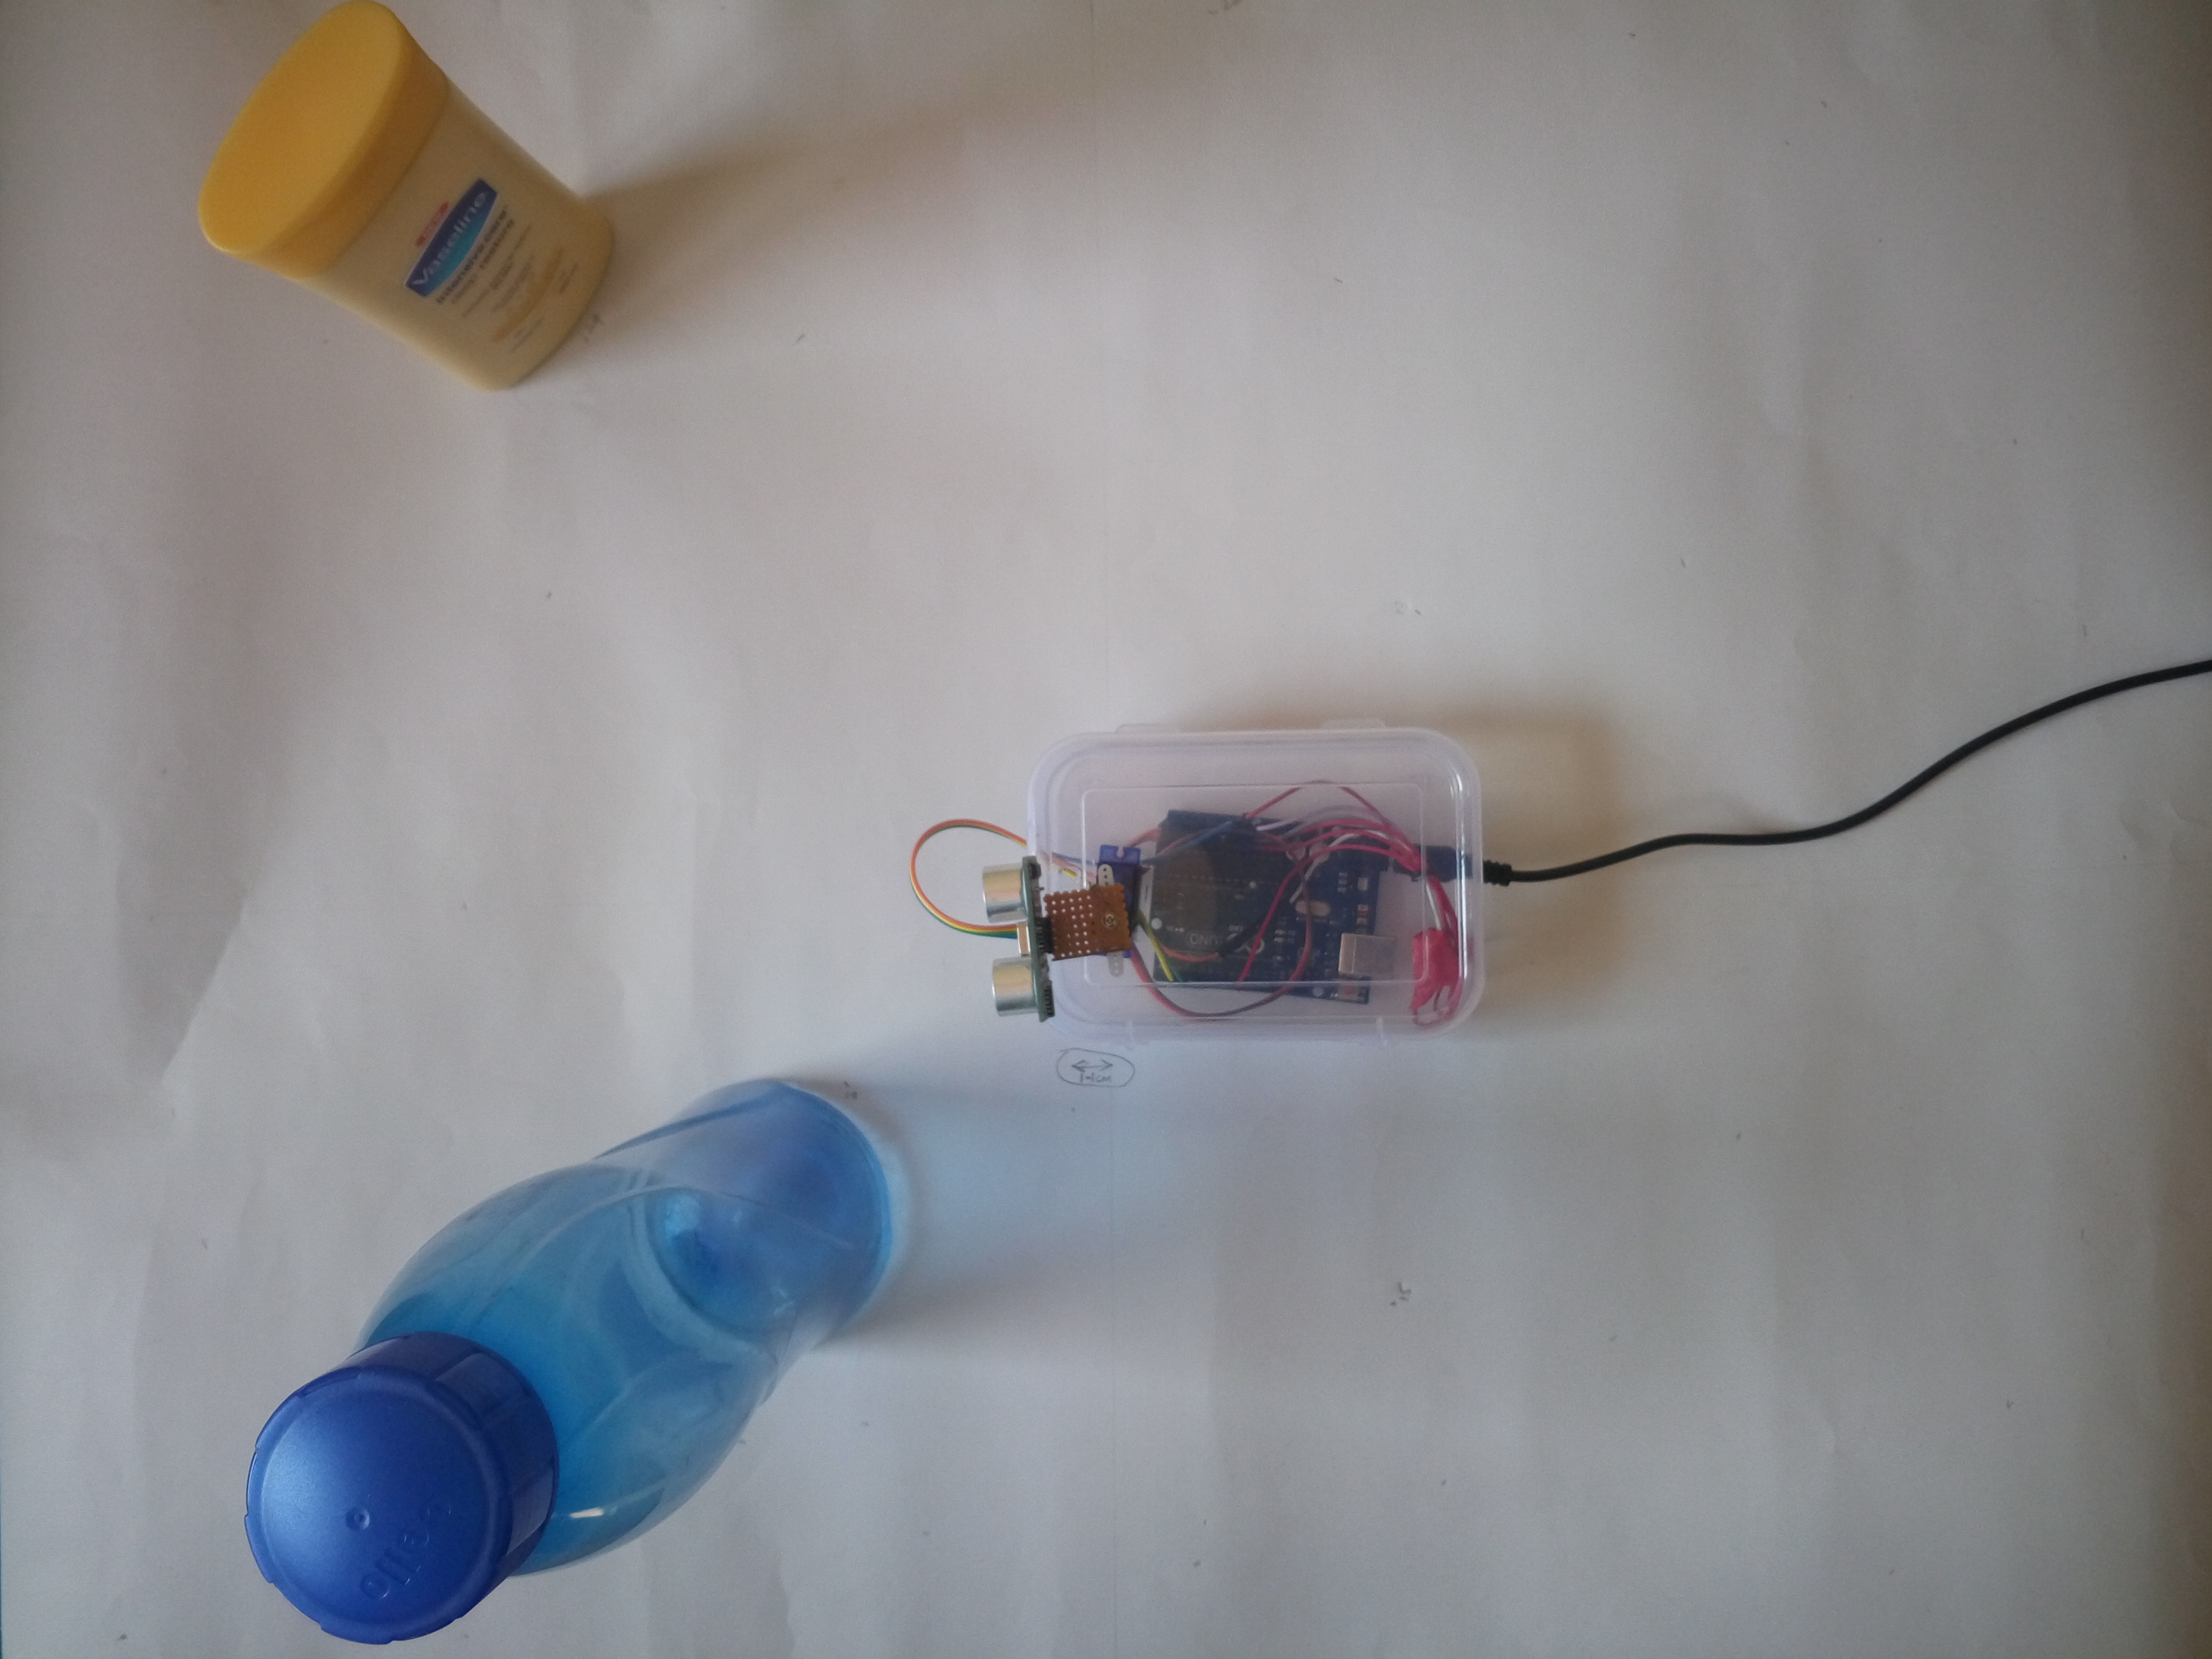
\includegraphics[width=0.4\textwidth]{../Files/project2.jpg}
	\caption{The project}  \label{fig:pro}
\end{figure}
\chapter{Appendix A : \arduino{} Code}\label{ch:appAlabel}
Here is the code uploaded on to the \arduinouno{}:
\begin{mdframed}[backgroundcolor=light-gray, roundcorner=10pt,leftmargin=1, rightmargin=1, innerleftmargin=15, innertopmargin=15,innerbottommargin=15, outerlinewidth=1, linecolor=light-gray]
\begin{lstlisting}[caption={The Arduino Code},language = C]
/*ver 1.1 (Final)*/

// Includes the Servo library
#include <Servo.h>. 

// Defines Trig and Echo pins of the Ultrasonic Sensor
const int trigPin = 2;
const int echoPin = 4;

// Variables for the duration & distance measured from the sensor
float duration;
float distance;

//Angle offset between graph and motor's XY axes
int offset = 0;
//Initial and final angles of motor's rotation
//Note that the motor can only take values 0-180.
//Make sure init_angle-offset >=60 to avoid jumper wire obstruction.
int init_ang = 70+offset;
int fin_ang = 180+offset;

// Declares a structure variable/object of the type Servo,
//(defined in the servo library) for controlling the servo motor.
Servo myServo; 

void setup() {
pinMode(trigPin, OUTPUT); // Sets the trigPin as an Output
pinMode(echoPin, INPUT); // Sets the echoPin as an Input
Serial.begin(9600); //Sets baud rate of serial communication
myServo.attach(9); // Defines on which pin is the servo motor attached
}

void loop() {
// if (Serial.available() > 0)  /*piece of code to be included in case of serial communication with IoT board*/
// {
// rotates the servo motor from init_ang to fin_ang degrees
for(int i=init_ang;i<=fin_ang;i++)
{  
myServo.write(i-offset);  //angle value to be passed to the servo library object for writing into the motor
delay(17);//DELAY #1:for time taken in motor rotation for one degree before calculating distance
distance = calculateDistance();// Calls a function for calculating the distance measured by the Ultrasonic sensor for each degree
Serial.print(i); // Sends the current degree into the Serial Port for graphical representation
Serial.print(","); // Sends addition character right next to the previous value needed later in the Processing IDE for indexing
Serial.print(distance); // Sends the distance value into the Serial Port for the graph
Serial.print(";"); // Sends addition character right next to the previous value needed later in the Processing IDE for indexing
}
// Repeats the previous lines from fin_ang to init_ang degrees
for(int i=fin_ang;i>init_ang;i--)
{  
myServo.write(i);
delay(17);  //DELAY #1 //can be minimised to 17 or 1667 microsec
distance = calculateDistance();
Serial.print(i);
Serial.print(",");
Serial.print(distance);
Serial.print(";");
}
//}
}
// Function for calculating the distance measured by the Ultrasonic sensor
float calculateDistance(){ 
unsigned long T1 = micros();
digitalWrite(trigPin, LOW); // trigPin needs a fresh LOW pulse before sending a HIGH pulse that can be detected from echoPin
delayMicroseconds(2);//DELAY #2:time for which low trig pulse is maintained before making it high
digitalWrite(trigPin, HIGH); 
delayMicroseconds(10);//DELAY #3:Sets the trigPin on HIGH state for 10 micro seconds
digitalWrite(trigPin, LOW);
duration = pulseIn(echoPin, HIGH); // Reads the echoPin, returns the sound wave travel time in microseconds
//distance= duration*0.034/2;
distance = (duration/2)/29.1;     //in cm,  datasheet gives "duration/58" as the formula

//To avoid sending data at variable time intervals due to varying time duration taken between execution of above code inside this function depending on distance of obstacle
//if no object, echo pulse is 38ms long HIGH
while(micros()-T1<38000)
{
;
}

return distance;
}
\end{lstlisting}

\end{mdframed}
\clearpage

\chapter{Appendix B : \processing{} Code}\label{ch:appAlabel}
The \emph{Java} code that we ran in \processing{} is given below :
\begin{mdframed}[backgroundcolor=light-gray, roundcorner=10pt,leftmargin=1, rightmargin=1, innerleftmargin=15, innertopmargin=15,innerbottommargin=15, outerlinewidth=1, linecolor=light-gray]
\begin{lstlisting}[caption={The Processing Code}, language=Java]
/*   Arduino Radar Project
*    1.1 [Final and complete]
*   Initialise every variable to null value to avoid null pointer exception
*/

import processing.serial.*; // imports library for serial communication
import java.awt.event.KeyEvent; // imports library for reading the data from the serial port
import java.io.IOException;

Serial myPort; // defines Object Serial
// defines variables
String angle="";
String distance="";
String data="";
String noObject="";
float pixsDistance=0.0;
int iAngle=0;
float iDistance=0.0;
int index1=0;
int index2=0;
int objCount=0,obctr=0;
PFont orcFont;
float angFlag=1.0;
float prevAng=0.0,deltaAng=0.0;
float maxDIST=50.0; //max distance of object in cms
int wctr=0;
float objWidth=0.0,prevWidth=0.0;
void setup() {

size (600, 700); // ***CHANGE THIS TO YOUR SCREEN RESOLUTION***
smooth();

myPort = new Serial(this,"/dev/ttyACM0", 9600); // Enter the COM Port address as COM4 or COM 22.starts the serial communication

myPort.bufferUntil('.'); // reads the data from the serial port up to the character '.'. So actually it reads this: angle,distance.
orcFont = loadFont("CenturySchL-Ital-20.vlw");

}

void draw() {

fill(237,13,245);
textFont(orcFont);
// simulating motion blur and slow fade of the moving line
noStroke();
fill(184,13); 
rect(0, 0, width, height-height*0.065); 

fill(211,27,228); //  color
// calls the functions for drawing the radar
drawRadar(); 
drawLine();
drawObject();
drawText();
}

void serialEvent (Serial myPort) { // starts reading data from the Serial Port
// reads the data from the Serial Port up to the character '.' and puts it into the String variable "data".
try{
data = myPort.readStringUntil(';');
data = data.substring(0,data.length()-1);

index1 = data.indexOf(","); // find the character ',' and puts it into the variable "index1"
angle= data.substring(0, index1); // read the data from position "0" to position of the variable index1 or thats the value of the angle the Arduino Board sent into the Serial Port
distance= data.substring(index1+1, data.length()); // read the data from position "index1" to the end of the data pr thats the value of the distance

// converts the String variables into Integer
iAngle = int(angle);
iDistance = float(distance);
deltaAng=iAngle-prevAng;

if(deltaAng*angFlag<0.0){
objCount=0;
objWidth=0;
}
//anticlockwise--deltaAng>0
//clockwise--deltaAng<0    
if(deltaAng>0.0)
angFlag=1.0;
else
angFlag=-1.0;
}
catch(Exception e){
println("Error parsing:");
e.printStackTrace();
}
}

void drawRadar() {
pushMatrix();
translate(width/2,height-height*0.507); // moves the starting coordinates to new location
noFill();
strokeWeight(2);
stroke(407,409,305);
// draws the arc lines
arc(0,0,(width-width*0.0385),(width-width*0.0385),PI,TWO_PI);
arc(0,0,(width-width*0.26),(width-width*0.26),PI,TWO_PI);
arc(0,0,(width-width*0.498),(width-width*0.498),PI,TWO_PI);
arc(0,0,(width-width*0.754),(width-width*0.754),PI,TWO_PI);
arc(0,0,(width-width*0.0385),(width-width*0.0385),0,PI);
arc(0,0,(width-width*0.26),(width-width*0.26),0,PI);
arc(0,0,(width-width*0.498),(width-width*0.498),0,PI);
arc(0,0,(width-width*0.754),(width-width*0.754),0,PI);
// draws the angle lines
line(-width/2,0,width/2,0);
line(0,0,(-width/2)*cos(radians(30)),(-width/2)*sin(radians(30)));
line(0,0,(-width/2)*cos(radians(60)),(-width/2)*sin(radians(60)));
line(0,0,(-width/2)*cos(radians(90)),(-width/2)*sin(radians(90)));
line(0,0,(-width/2)*cos(radians(120)),(-width/2)*sin(radians(120)));
line(0,0,(-width/2)*cos(radians(150)),(-width/2)*sin(radians(150)));
line(0,0,(-width/2)*cos(radians(180)),(-width/2)*sin(radians(180)));
line(0,0,(-width/2)*cos(radians(210)),(-width/2)*sin(radians(210)));
line(0,0,(-width/2)*cos(radians(240)),(-width/2)*sin(radians(240)));
line(0,0,(-width/2)*cos(radians(270)),(-width/2)*sin(radians(270)));
line(0,0,(-width/2)*cos(radians(300)),(-width/2)*sin(radians(300)));
line(0,0,(-width/2)*cos(radians(330)),(-width/2)*sin(radians(330)));
line((-width/2)*cos(radians(30)),0,width/2,0);
popMatrix();
}

void drawLine() {
pushMatrix();
strokeWeight(8);
stroke(32,65,174); //color for blue line
translate(width/2,height-height*0.507); // moves the starting coordinates to new location
line(0,0,(height-height*0.575)*cos(radians(iAngle)),-(height-height*0.575)*sin(radians(iAngle))); // draws the line according to the angle
popMatrix();
}

void drawObject() {
pushMatrix();
translate(width/2,height-height*0.508); // moves the starting coordinats to new location
strokeWeight(8);
stroke(240,1,40); // red color
pixsDistance = iDistance*((height-height*0.1666)*0.013/3); // covers the distance from the sensor from cm to pixels
if(iDistance<=maxDIST){
if(wctr>2){    //Assuming that an object will be thick enough to be detected for 2 degrees of rotation.
objWidth=0.0;
// draws the object according to the angle and the distance
line(pixsDistance*cos(radians(iAngle)),-pixsDistance*sin(radians(iAngle)),(width-width*0.505)*cos(radians(iAngle)),-(width-width*0.505)*sin(radians(iAngle)));
obctr++;
}
}
popMatrix();
}

void drawText() { // draws the texts on the screen
pushMatrix();
if(iDistance>maxDIST) {
noObject = "No object within Range";
if(wctr==0)
objWidth=prevWidth;
else
objWidth=float(wctr)*iDistance*0.0174;  //width of object in cm
prevWidth=objWidth;
wctr=0;
if(obctr>0){
objCount++;
obctr=0;
}
}
else {
wctr++;
if(wctr>2)  //Assuming that an object will be thick enough to be detected for 2 degrees of rotation.
{
noObject = "Object in Range";

}
} 

fill(0,0,0);  //black background of bottom text
noStroke();
rect(0, height-height*0.0521, width, height);
fill(251,255,249);
textSize(15);

text("30cm",width-width*0.4041,height-height*0.4793);
text("60cm",width-width*0.281,height-height*0.4792);
text("90cm",width-width*0.177,height-height*0.4792);
text("120cm",width-width*0.0729,height-height*0.4792);
textSize(16);
text(noObject, width-width*0.634, height-height*0.0218);
text("Angle: " + iAngle +" @\degree@", width-width*0.97, height-height*0.0232);
text("Distance: ", width-width*0.26, height-height*0.0235);
textSize(16);
text(" No. of objects: "+ objCount +"", width-width*0.986, height-height*0.0714);
text(" Object Width: "+ objWidth +"", width-width*0.986, height-height*0.1714);
if(iDistance<=maxDIST) {
if(wctr>2)
text("        " + iDistance + " cm", width-width*0.185, height-height*0.0237);
}
textSize(19);
fill(7,7,6); //color for degrees text
translate((width-width*0.5020)+width/2*cos(radians(30)),(height-height*0.5283)-width/2*sin(radians(30)));
rotate(-radians(-60));
text("30@\degree@",0,0);
resetMatrix();
translate((width-width*0.507)+width/2*cos(radians(60)),(height-height*0.5139)-width/2*sin(radians(60)));
rotate(-radians(-29));
text("60@\degree@",-4,-5);
resetMatrix();
translate((width-width*0.507)+width/2*cos(radians(90)),(height-height*0.5149)-width/2*sin(radians(90)));
rotate(radians(0));
text("90@@\degree@@",-5,-2);
resetMatrix();
translate(width-width*0.513+width/2*cos(radians(120)),(height-height*0.51286)-width/2*sin(radians(120)));
rotate(radians(-30));
text("120@\degree@",0,0);
resetMatrix();
translate((width-width*0.5298)+width/2*cos(radians(150)),(height-height*0.4803)-width/2*sin(radians(150)));
rotate(radians(-60));
text("150@\degree@",0,0);
resetMatrix();
translate(width-width*0.475+width/2*cos(radians(180)),(height-height*0.47791)-width/2*sin(radians(180)));
rotate(radians(-90));
text("180@\degree@",0,0);
resetMatrix();
translate(width-width*0.494+width/2*cos(radians(210)),(height-height*0.4797)-width/2*sin(radians(210)));
rotate(radians(-120));
text("210@\degree@",0,0);
resetMatrix();
translate(width-width*0.484+width/2*cos(radians(240)),(height-height*0.4867)-width/2*sin(radians(240)));
rotate(radians(-150));
text("240@\degree@",0,0);
resetMatrix();
translate(width-width*0.474+width/2*cos(radians(270)),(height-height*0.50151)-width/2*sin(radians(270)));
rotate(radians(-180));
text("270@\degree@",0,0);
resetMatrix();
translate(width-width*0.470+width/2*cos(radians(300)),(height-height*0.51167)-width/2*sin(radians(300)));
rotate(radians(-210));
text("300@\degree@",0,0);
resetMatrix();
translate(width-width*0.478+width/2*cos(radians(330)),(height-height*0.5174)-width/2*sin(radians(330)));
rotate(radians(-240));
text("330@\degree@",0,0);
resetMatrix();
translate(width-width*0.523+width/2*cos(radians(360)),(height-height*0.52132)-width/2*sin(radians(360)));
rotate(radians(-270));
text("0@\degree@",0,0);
popMatrix(); 
prevAng = iAngle;
}
\end{lstlisting}
\end{mdframed}
\clearpage
\end{document}
